% $Log$
% Revision 1.8  2006/02/11 13:00:05  kelsaka
% - anhang ausgegliedert
%
% Revision 1.7  2006/02/11 10:02:08  kelsaka
% - appendix angef�gt
%
% Revision 1.6  2006/02/10 19:15:26  kelsaka
% - pagestyle ge�ndert
%
% Revision 1.5  2006/02/10 19:07:23  kelsaka
% - auf buch-dokument-typ gewechselt
%
% Revision 1.4  2006/01/25 14:43:00  kelsaka
% - titelfolie: datum
% - mehrfache-delegation bei assembly konnektoren
%
% Revision 1.3  2006/01/22 13:09:02  kelsaka
% - anotation --> annotation
%
% Revision 1.2  2006/01/15 13:43:23  kelsaka
% - allokation, assembly, deployment, ...
%
% Revision 1.1  2006/01/05 16:46:14  kelsaka
% - initial creation
%


\documentclass[12pt]{scrbook} %scrartcl

\usepackage[a4paper,left=3.0cm,right=2.5cm,top=3.0cm,bottom=2.5cm,headheight=15pt,headsep=1.5cm,footskip=1cm]{geometry}

%---- Sonderzeichen-------%
\usepackage {ngerman}
\usepackage{umlaut}
%---- Codierung----%
\usepackage[latin1]{inputenc}	% f�r Unix und Windows
%\usepackage[applemac]{inputenc}	% f�r MAC

%----- Mathematischer Zeichenvorrat---%
\usepackage{amsmath}
\usepackage{amssymb}

%----- Graphik ------%
\usepackage{graphicx}
%\usepackage[pdftex]{graphics}
\usepackage{makeidx}

\usepackage{enumerate}

% fuer die aktuelle Zeit
\usepackage{scrtime}



%\usepackage{hyperref}
%\usepackage{lastpage}       % Seitennummer der letzten Seite auslesen

\usepackage[colorlinks=true, pdfstartview=FitV, linkcolor=black,
citecolor=black, urlcolor=black]{hyperref}



\usepackage{fancyhdr}
\lhead{\nouppercase{\leftmark}} \chead{} \rhead{\thepage}
\fancyfoot {}

\makeindex
%Glossar
\usepackage{nomencl}
\let\abbrev\nomenclature
\renewcommand{\nomname}{Glossar}
\setlength{\nomlabelwidth}{.25\hsize}
\renewcommand{\nomlabel}[1]{#1 \dotfill}
\setlength{\nomitemsep}{-\parsep}
\makeglossary


\usepackage[normalem]{ulem}
\newcommand{\markup}[1]{\uline{#1}}

\begin{document}
	
	% Trennungen
	\hyphenation{Wort-um-bruch}
\hyphenation{Kom-po-nen-ten-mo-dell}
\hyphenation{Trans-for-ma-tions-an-wei-sun-gen}
\hyphenation{Trans-for-ma-tions-an-wei-sung}
% \hyphenation{Un-ter-st"ut-zung}
\hyphenation{Mo-dell}
\hyphenation{Con-straints}
\hyphenation{Grund-an-nah-men}
\hyphenation{Grund-an-nah-me}
\hyphenation{Pro-jekt-ri-si-ken}
% \hyphenation{be-n\"o-tig-ten}
\hyphenation{Schnitt-stel-le}
\hyphenation{Con-nec-tor}
	
	% Titelblatt
	%
% This file has been generated by UML to LaTeX written in oAW Xpand
% It is save to alter this file as it WILL NOT be overwritten.
% The file is included by the main latex file in the appropriate place, not further
% actions are required
%


	% Pagecounter auf 2 Setzen
	\setcounter{page}{2}
	
	\setcounter{secnumdepth}{3}
	
	% Inhaltsverzeichnis
	\tableofcontents
	
	%	leere Seite nach TOC
	%\pagebreak
	%\newpage
	%$\,$


	% Fancyheader setzen
	%\pagestyle{fancy}
		
	%Inhalt
	% $Log$
% Revision 1.26  2006/01/15 13:43:23  kelsaka
% - allokation, assembly, deployment, ...
%
% Revision 1.25  2006/01/15 11:21:23  kelsaka
% - kleinere erg�nzungen
%
% Revision 1.24  2006/01/14 19:18:35  kelsaka
% - inhaltsstruktur erg�nzt
%
% Revision 1.23  2006/01/14 18:20:07  kelsaka
% - sub-typ-beschreibungen vervollst�ndigt
%
% Revision 1.22  2006/01/14 17:04:04  kelsaka
% - trivial protokoll eingf�hrt
%
% Revision 1.21  2006/01/14 15:00:05  kelsaka
% - komponenten-substitution
%
% Revision 1.20  2006/01/14 13:14:14  kelsaka
% - sub-typ beziehung erg�nzt
%
% Revision 1.19  2006/01/14 11:46:03  kelsaka
% - sub-typ-beispiel �berarbeitet und erkl�rt
%
% Revision 1.18  2006/01/14 10:58:34  kelsaka
% - SEFFs: Pr�zisierung
%
% Revision 1.17  2006/01/13 18:58:05  kelsaka
% - abschluss der typ-beschreibung
%
% Revision 1.16  2006/01/13 17:07:21  kelsaka
% - weitere erg�nzung
%
% Revision 1.15  2006/01/13 16:25:16  kelsaka
% - ebenen-beziehungen erg�nzt
%
% Revision 1.14  2006/01/13 15:52:43  kelsaka
% - komponenten-typen: beschreibung erg�nzt
%
% Revision 1.13  2006/01/13 12:47:27  kelsaka
% - seff-berechnung erg�nzt
%
% Revision 1.12  2006/01/13 08:06:44  kelsaka
% - protokollberechnung erg�nzt
%
% Revision 1.11  2006/01/12 09:43:53  kelsaka
% - pr�zisierungen eingef�gt
%
% Revision 1.10  2006/01/11 17:18:05  kelsaka
% - beschreibung des komponentenmodells erg�nzt
%
% Revision 1.9  2006/01/11 16:19:45  kelsaka
% - beschreibung des komponentenmodells erg�nzt
%
% Revision 1.8  2006/01/09 16:47:45  kelsaka
% - Kapitel erg�nzt
%
% Revision 1.7  2006/01/09 14:28:51  kelsaka
% - beschreibung des komponentenmodells weiter erg�nzt
% - alte inhalte (aus prosposal) weitestgehend entfernt
%
% Revision 1.6  2006/01/09 13:26:55  kelsaka
% - beschreibung des komponentenmodells erg�nzt
%
% Revision 1.5  2006/01/09 09:49:10  kelsaka
% - beschreibung des komponentenmodells weiter erg�nzt
%
% Revision 1.4  2006/01/08 17:43:03  kelsaka
% - beschreibung des komponentenmodells weiter erg�nzt
%
% Revision 1.3  2006/01/08 15:42:41  kelsaka
% - beschreibung des komponentenmodells erg�nzt
%
% Revision 1.1  2006/01/05 16:46:14  kelsaka
% - initial creation
%


% TODO: auf rechte Seite pr�fen --> je nach TOC
\section{Abstract}
\label{sec:Abstract}
\begin{abstract}
	TODO: Abstract
\end{abstract}

\newpage
%	leere Seite
$\,$
\newpage



\section{Einleitung}
\label{sec:Einleitung}



\subsection{�berblick}
\label{sec:EinleitungUeberblick}



\subsection{Bemerkungen}
\label{sec:EinleitungBemerkungen}
Ist im Folgenden von \textit{Komponentenmodell} die Rede, so ist, sofern nicht anders angegeben, das \textit{Palladio Komponentenmodell} gemeint. Als Palladio Komponentenmodell wird dabei das \textit{Meta}-Modell zur Darstellung von Komponentenarchitekturen der Palladio-Gruppe \cite{PALL} bezeichnet. Dieses Modell wird in Kapitel \ref{sec:DasPalladioKomponentenmodell} n�her beschrieben.

Zudem bezeichnet der Begriff \textit{Projekt}, solange er ohne sonstigen Kontext verwendet wird, die Diplomarbeit.



\section{Das Palladio Komponentenmodell}
\label{sec:DasPalladioKomponentenmodell}
Im Rahmen der Diplomarbeit wird ein Meta-Modell f�r das Palladio Komponentenmodell erstellt. Daher ist es unabdingbar, dass ein vollst�ndiges Verst�ndnis f�r das Komponentenmodell existiert. Die folgenden Kapitel zeigen detailliert die Eigenschaften des Komponentenmodells auf. Schlie�lich wird dem gegen�bergestellt, welche Konzepte des Komponentenmodells umgesetzt werden konnten, welche Einschr�nkungen bei der Modellierung auftraten und welche \textit{Work"=Arounds} aus welchen Gr�nden zur Abbildung notwendig waren.

Das im Folgenden dargestellte Palladio Komponentenmodell entspricht dem Stand der Konzepte des Januars 2006.



\subsection{Einfache Komponenten}
\label{sec:EinfacheKomponenten}



\begin{figure}[htbp]
	\centering
		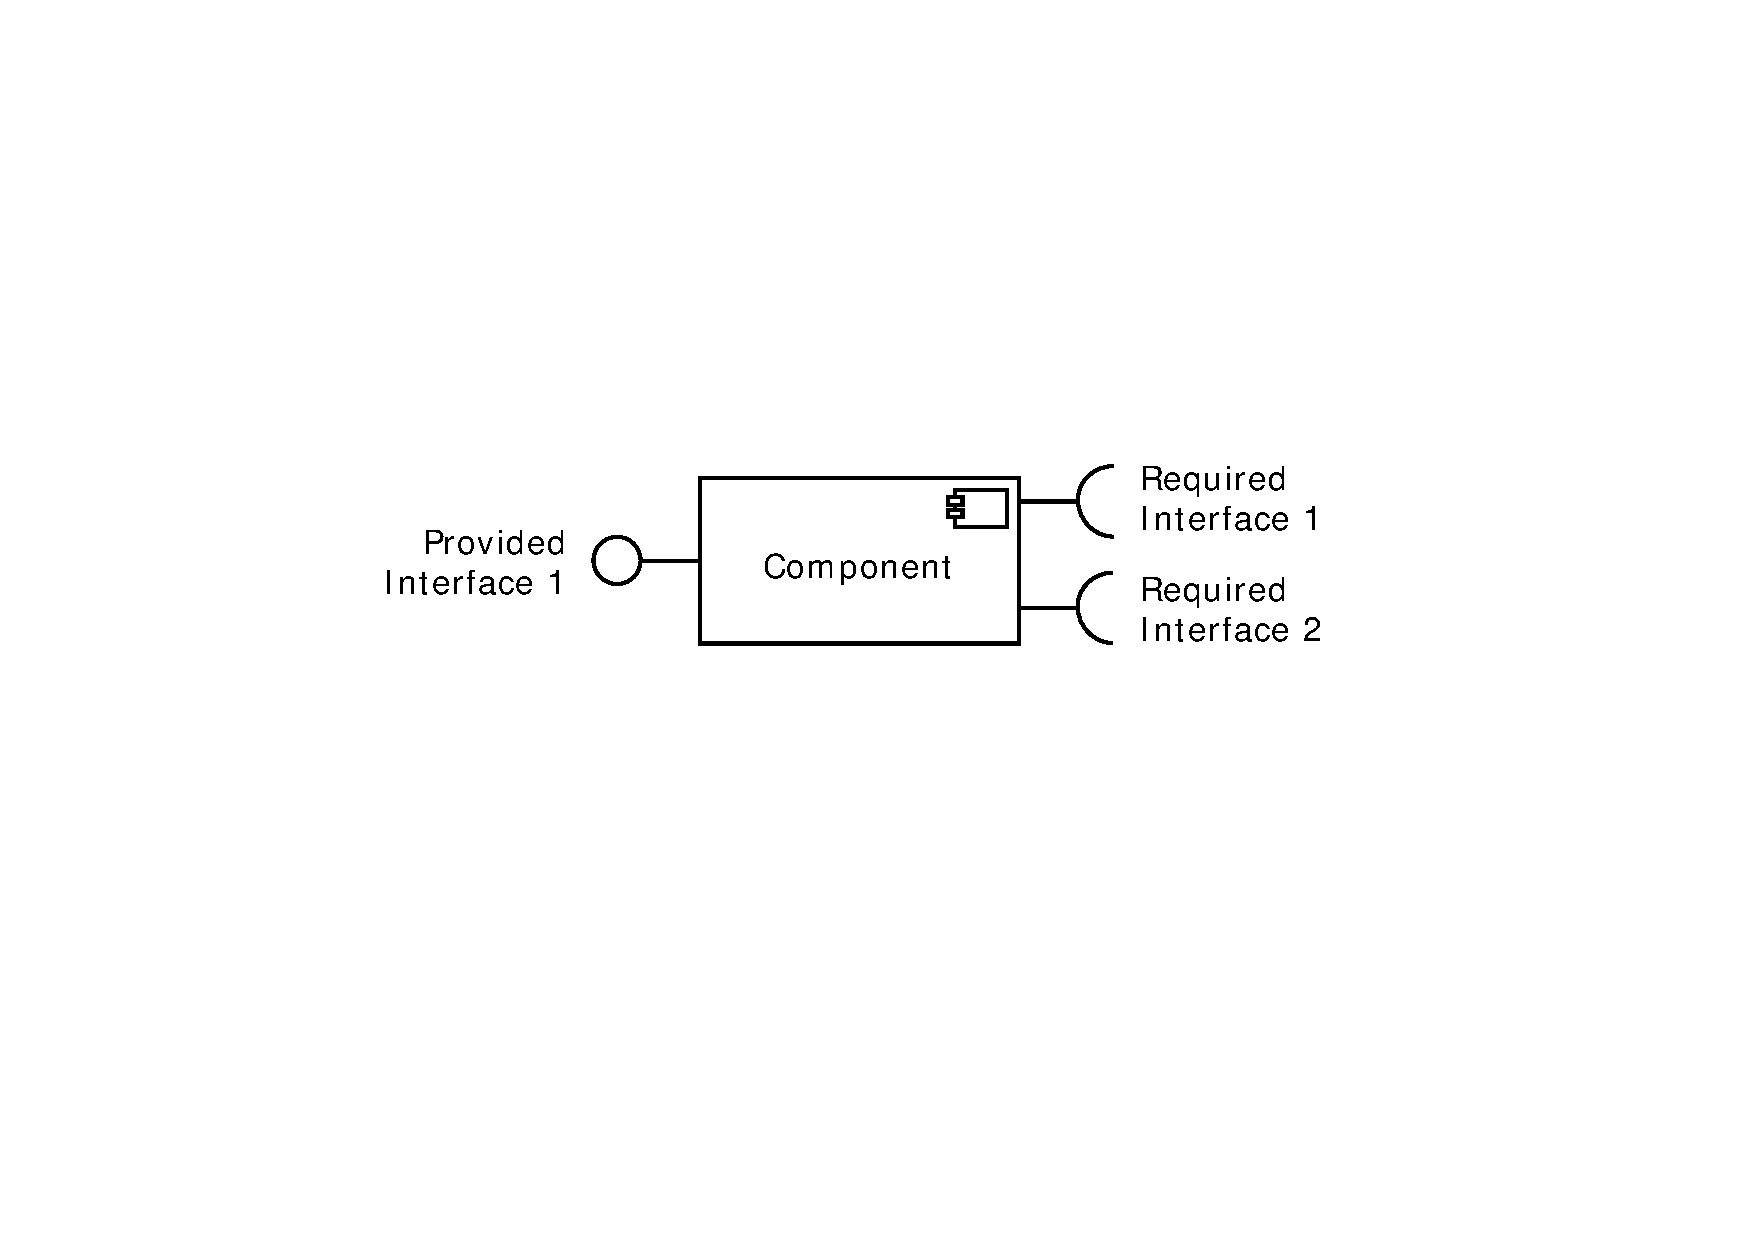
\includegraphics[width=0.70\textwidth]{./image/cm-simple-component-01.pdf}
	\caption{Einfache Komponente mit einer angebotener und zwei be\-n�\-tig\-ten Schnittstellen}
	\label{fig:cm-simple-component-01}
\end{figure}



Das Palladio Komponentenmodell -- unter \cite{BECK} findet sich die Beschreibung einer �lteren Fassung des Modells -- beschreibt Software-Architekturen als eine Menge von Komponenten und Schnittstellen, sowie darauf definierten Relationen. In Abbildung \ref{fig:cm-simple-component-01} wird eine einfache Komponente "`Component"' gezeigt, die eine Schnittstelle anbietet (\textit{Provided Interface}), im Beispiel "`Provided Interface 1"' genannt. Daneben ben�tigt die Komponente zwei Schnittstellen ("`Required Interface 1 / 2"').

Im Folgenden sollen zun�chst einfache Basiskonstrukte des Komponentenmodell dargestellt werden. Eine detaillierte Erkl�rung, welche Konstrukte in welchen Situationen als valide bewertet werden, folgt in den n�chsten Kapiteln (ref TODO: Kapitelnummer). In den Abbildungen dieses Kapitel wird auf die standardisierte Visualisierung mit Hilfe von UML 2 Komponentendiagrammen \cite{uml2} zur�ckgegriffen.

Eine Komponente kann \texttt{0..*} Schnittstellen anbieten. Das bedeutet, dass die Komponenten die Dienste auch anbieten muss, die �ber eine Schnittstelle festgelegt sind. Der Aufbau einer Schnittstelle wird in Kapitel ref{TODO} beschrieben. F�r eine Komponente darf im Allgemeinen jedoch nicht angenommen werden, das angebotene Schnittstellen und darauf definierte Dienste auch tats�chlich angesprochen werden.

Auf der \textit{Requires}-Seite ist eine Komponente ebenso frei und kann \texttt{0..*} Schnittstellen ben�tigen. Durch die \textit{Requires}-Schnittstelle definiert eine Komponente die Dienste, die sie selbst ben�tigt. Wird eine Komponente verwendet, muss f�r eine vollst�ndige uneingeschr�nkte Verwendung sichergestellt werden, dass die ben�tigten Dienste ebenso vollst�ndig von anderen Komponenten angeboten werden und erreicht werden k�nnen (zur Verbindung zwischen Komponenten siehe Kapitel ref{TODO}).

Eine Komponente kann im �brigen die gleiche Schnittstelle anbieten und zugleich verlangen. Stellt man sich beispielsweise eine \textit{Chain-of-Responsibility} (vgl. \cite{GAMMA}) vor, die �ber Komponenten realisiert wird, so wird die gleiche Schnittstelle zur Annahme (\textit{provided}) von Dienstaufrufen und zur Weitergabe von Dienstaufrufen an den Nachfolger in der Kette verwendet.



\subsection{Schnittstellen und Rollen}
\label{sec:SchnittstellenUndRollen}



\begin{figure}[htbp]
	\centering
		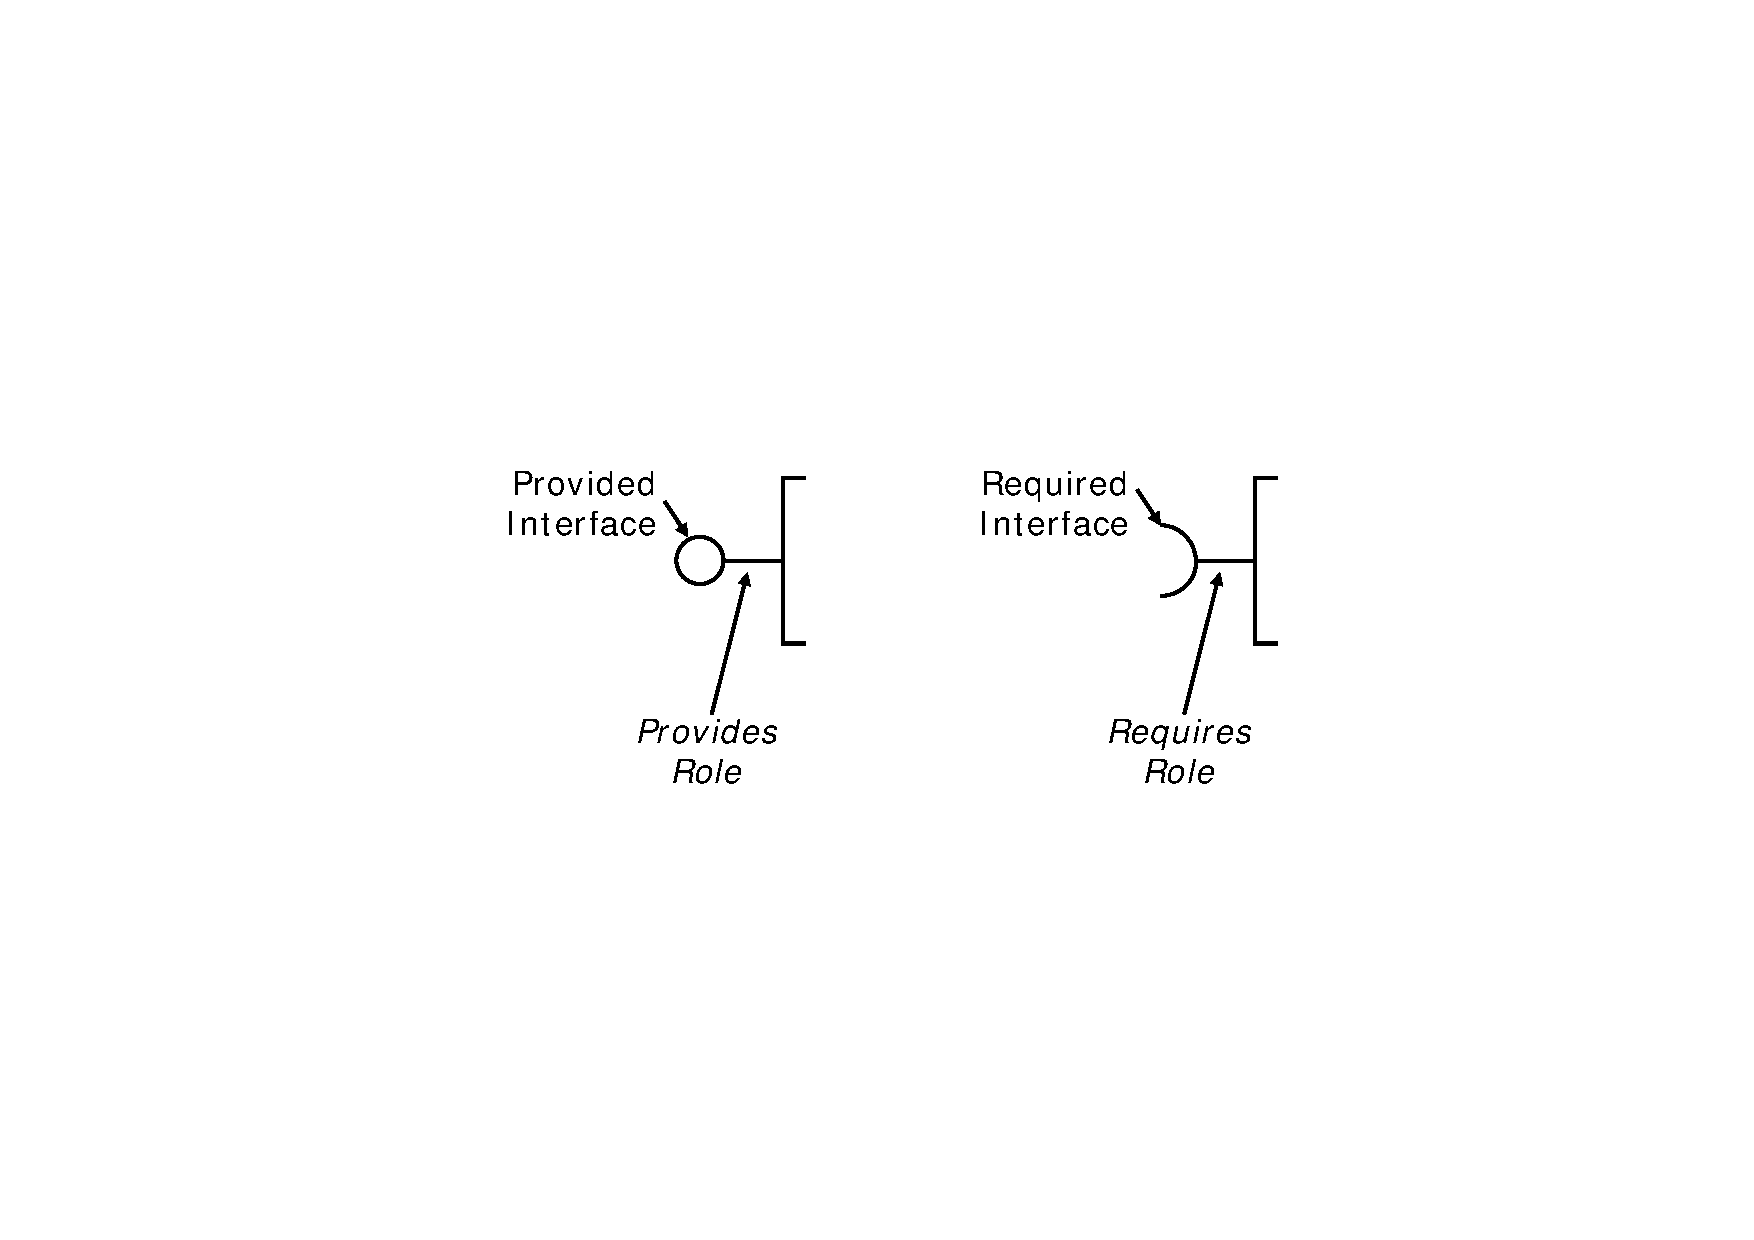
\includegraphics[width=0.55\textwidth]{./image/cm-interfaces-roles-01.pdf}
	\caption{Angebotene und ben�tigte Schnittstellen mit ihren dazugeh�rigen Rollen in UML2"=Notation}
	\label{cm-interfaces-roles-01}
\end{figure}



�ber Abbildung \ref{cm-interfaces-roles-01} soll verdeutlicht werden, welche Bestandteile der graphischen Notation, die auch im Folgenden verwendet wird, einem Interface entsprechen. Auf der linken Seite ist eine Komponente angedeutet, die eine Schnittstelle anbietet. Bietet eine Komponente eine Schnittstelle an (\textit{Provided Interface}), so impliziert dies, dass eine \textit{Provides Role} zwischen Komponente und Interface existiert. In der graphischen Notation ist die vergleichbar mit der Verbindungslinie zwischen Schnittstelle und Komponente. Wird eine Komponente angeboten, resultiert dies in einer Kreisdarstellung f�r die Schnittstelle.

Auf der rechten Seite der Abbildung ist die \textit{Requires Role} zwischen einer Komponente unter der Schnittstelle dargestellt. Auch hier entspricht die Verbindungslinie zwischen Komponente und Schnittstelle der Rollen-Beziehung. Die graphische Notation �ndert sich jedoch. Aus dem Kreis, der die Schnittstelle symbolisiert, wird ein Halbkreis.

Auch im Komponentenmodell wird die Relation zwischen Komponente und Schnittstelle als "`Rolle"' (\textit{Role}) bezeichnet. Die Art der Rolle (angeboten oder ben�tigt / \textit{provided} oder \textit{required}) entscheidet �ber die Verwendung der Schnittstelle. Die Eigenschaft der Schnittstelle selbst �ndert sich jedoch nicht durch ihre Verwendung. Auch in Abbildung \ref{cm-interfaces-roles-01} k�nnten die Komponenten die beiden dargestellten Schnittstellen identisch sein.

Eine Schnittstelle wird also erst durch eine \textit{Provides Role} zu einer angebotene Schnittstelle / einem \textit{Provided Interface}, bzw. �ber eine \textit{Requires Role} zu einer ben�tigten Schnittstelle / einem\textit{Required Interface}.



\subsection{Assembly Konnektoren}
\label{sec:Assembly Konnektoren}



\begin{figure}[htbp]
	\centering
		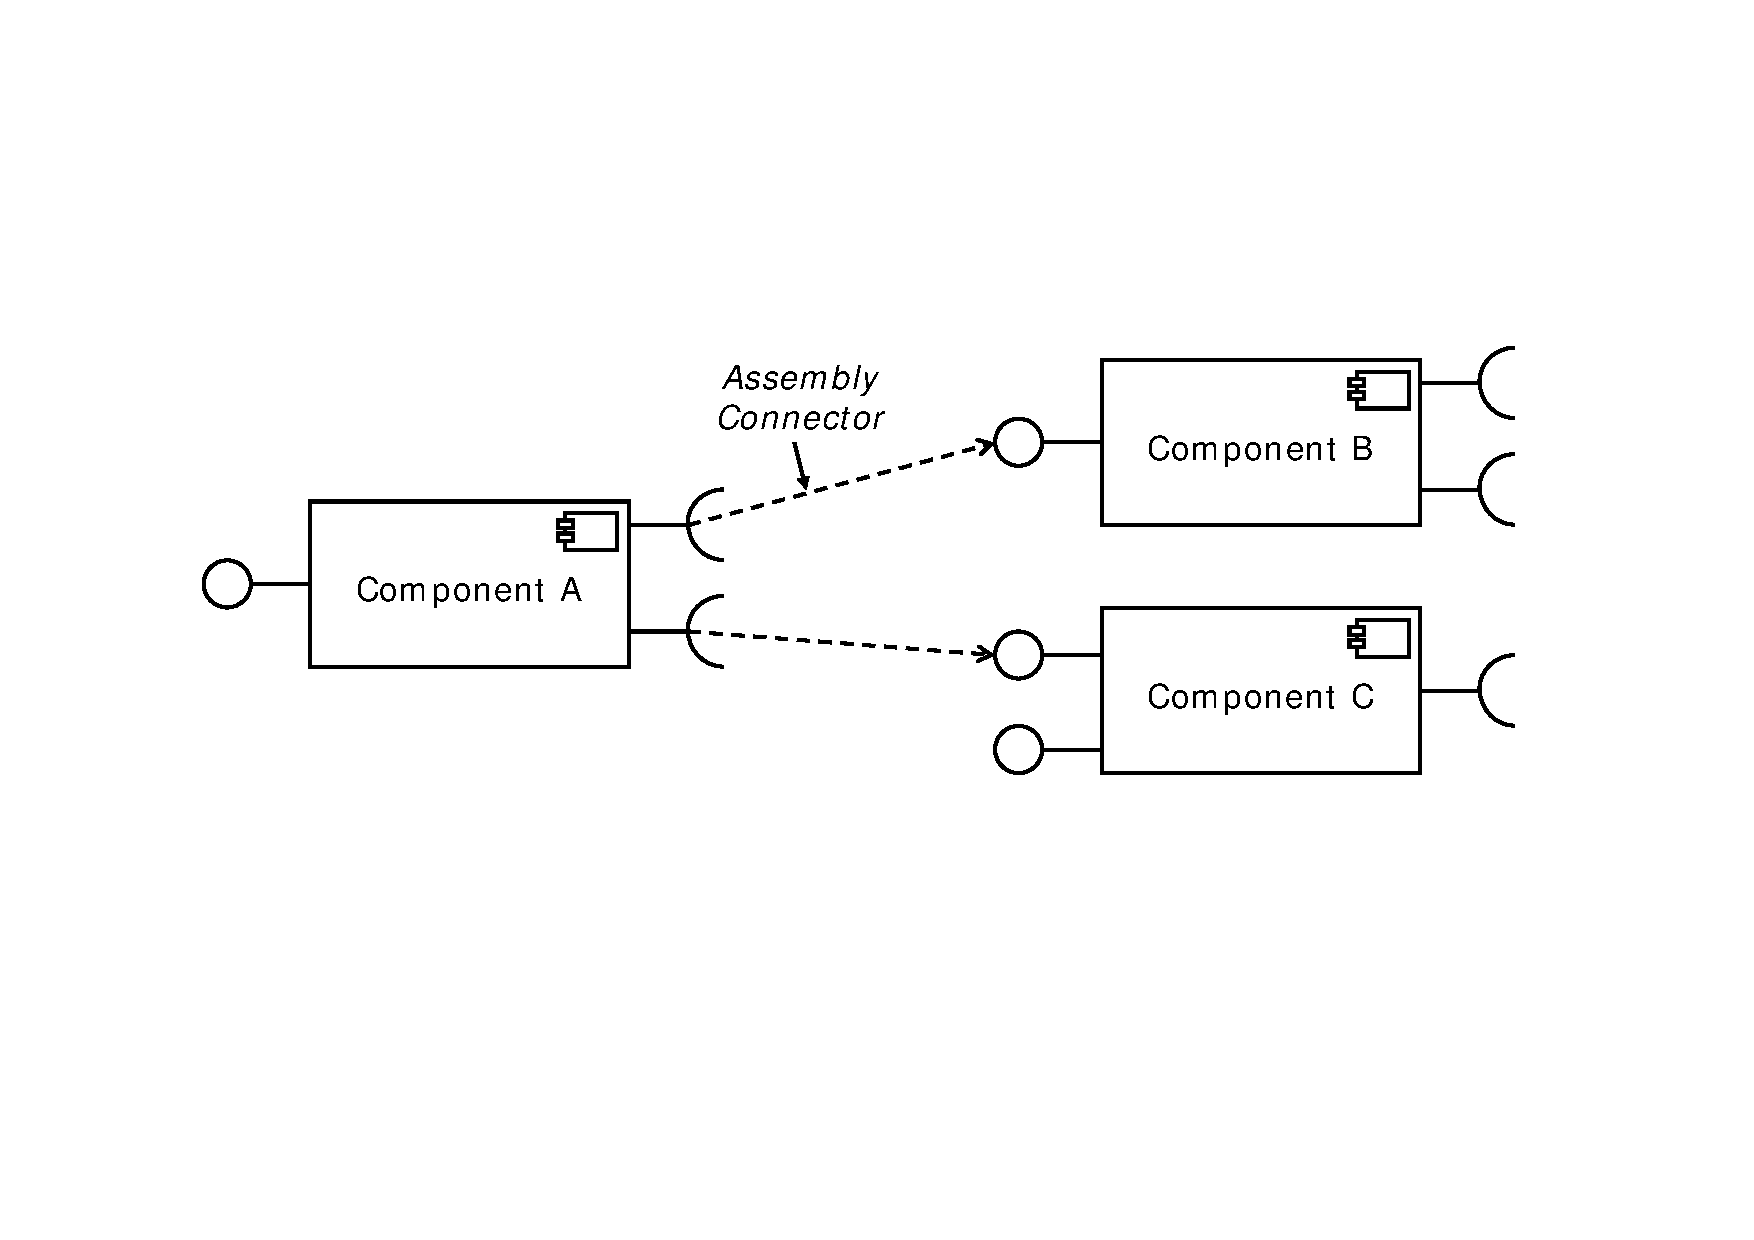
\includegraphics[width=1.00\textwidth]{./image/cm-assembly-connector-01.pdf}
	\caption{Eine Komponente wird �ber Assembly Konnektoren mit zwei weiteren Komponenten verbunden}
	\label{fig:cm-assembly-connector-01}
\end{figure}



In Abbildung \ref{fig:cm-assembly-connector-01} wird die Verwendung zweier Assembly Konnektoren (\textit{Assembly Connector}) dargestellt. Pr�zise betrachtet verbinden Assembly Konnektoren je eine angebotene (\textit{Provides Role}) und eine ben�tigte Rolle (\textit{Requires Role}) einer Schnittstelle. Dies bedeutet, dass Aufrufe der �ber die \textit{Requires Role} mit der ben�tigten Schnittstelle verbundenen Komponente auf die angebotene Schnittstelle und damit auf die �ber eine \textit{Provides Role} damit verbundene Komponente weitergeleitet werden. Der Kontrollflu� folgt damit in diesem Fall der als gestrichelt dargestellten Linie in Pfeilrichtung.

Jede ben�tigte Schnittstelle einer Komponente wird damit mit genau einer angebotenen Schnittstelle verbunden. Sind die angebotene Schnittstelle und die ben�tigte Schnittstelle einer Komponente identisch oder kompatibel (Def. siehe TODO), so kann eine Komponente grunds�tzlich auch eigene Dienste aufrufen. In der noch folgenden Differenzierung �ber die Typ-Ebenen des Komponentenmodells (siehe Kapitel \ref{sec:Typ-Ebenen}) wird deutlich, weshalb dies nicht zwangsl�ufig zu einer infiniten Rekursion f�hren muss.



\subsection{Zusammengesetzte Komponenten}
\label{sec:ZusammengesetzteKomponenten}



\begin{figure}[htbp]
	\centering
		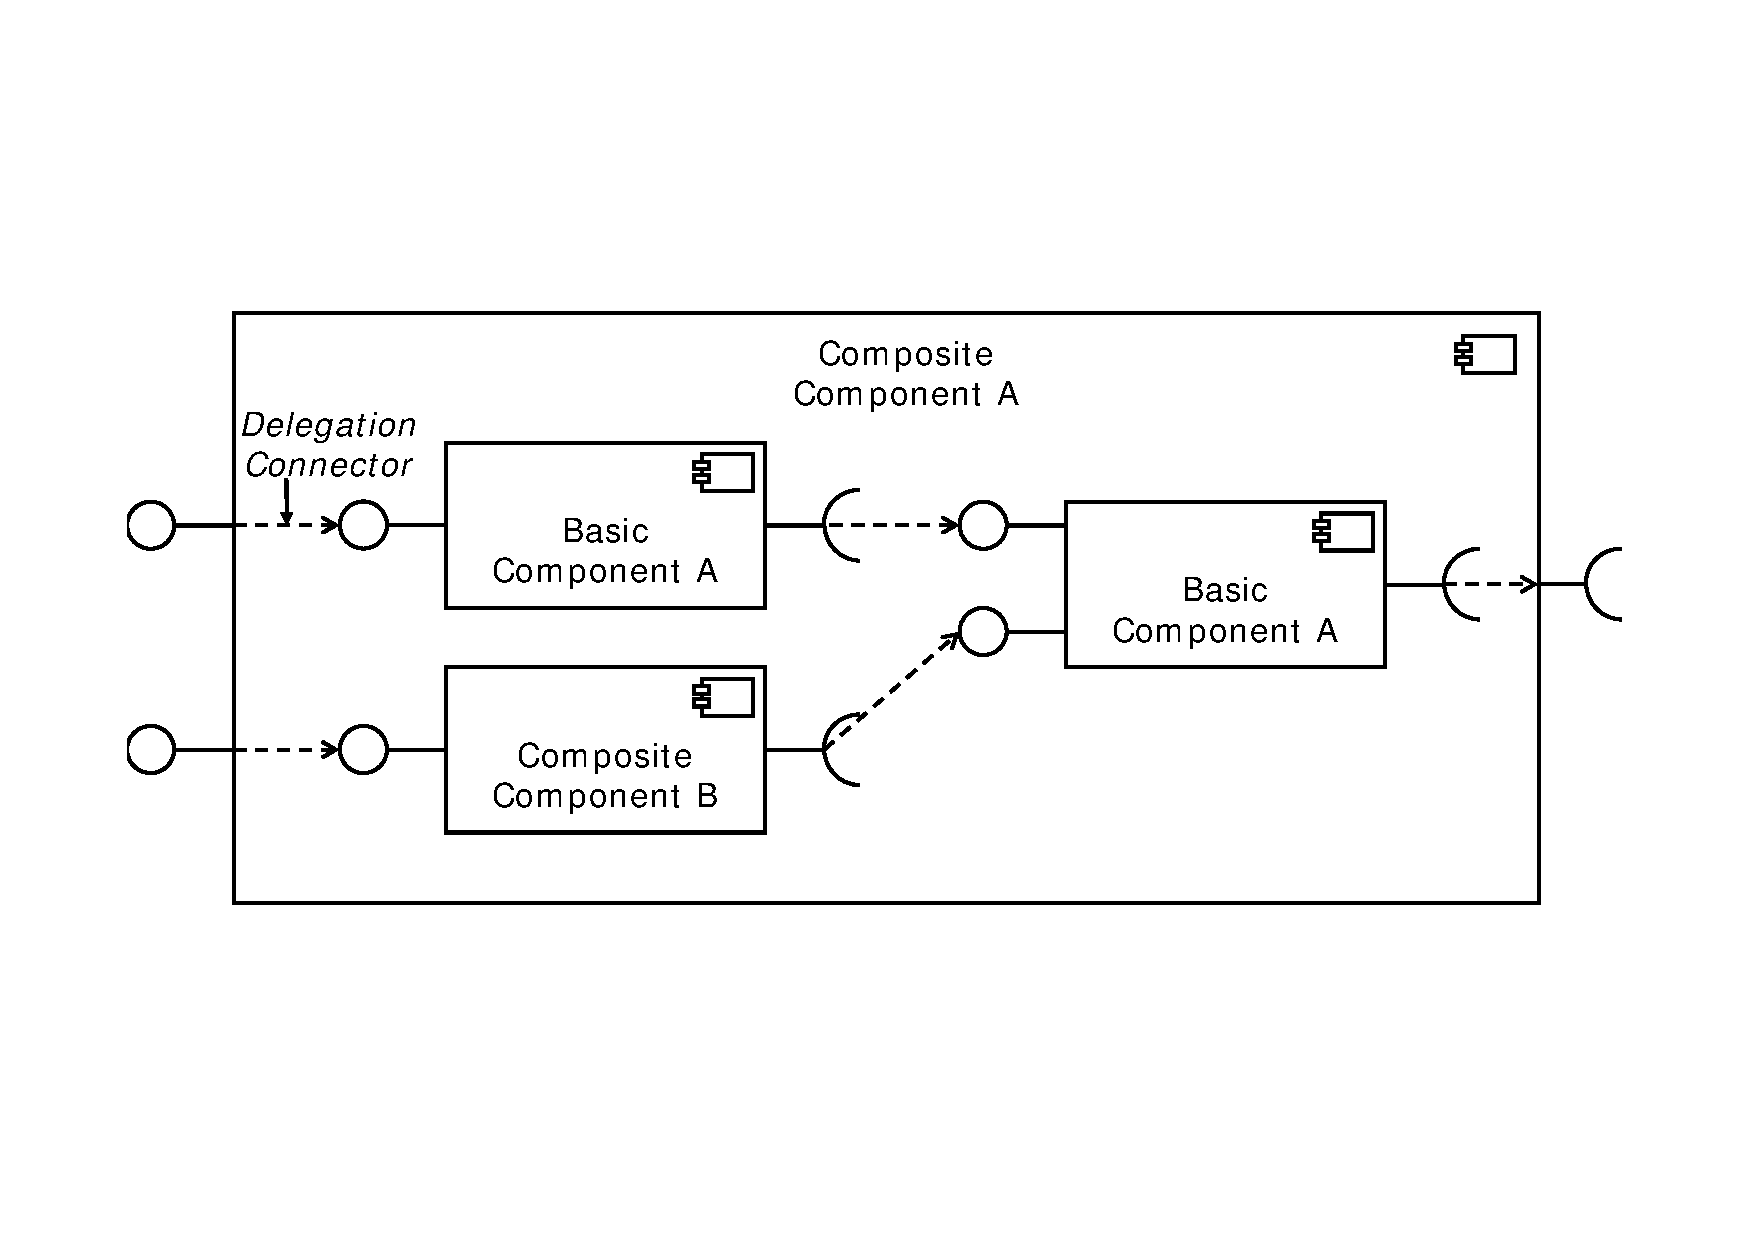
\includegraphics[width=1.00\textwidth]{./image/cm-composite-component-01.pdf}
	\caption{Eine zusammengesetzte Komponente mit inneren Komponenten}
	\label{fig:cm-composite-component-01}
\end{figure}



Zusammengesetzte Komponenten, im Folgenden auch \textit{Composite Components} genannt, enthalten eine interne Realisierung �ber weitere Komponenten und �ber zugeh�rige Strukturen. Ein \textit{Composite Component} selbst enth�lt keine Realisierung etwa �ber Quellcode, sondern fasst eine logisch und / oder funktional zusammengeh�rige Menge von Komponente zusammen. �ber diesen Mechanismus lassen sich Hierarchien von Komponenten definieren. Zudem stellt eine Composite Component eine Abstraktion und Kapselung ihres Innenlebens (\textit{Information Hiding}) zur Verf�gung, wenn sie nur �ber die �u�eren Schnittstellen betrachtet wird (TODO: weitere Konzeptideen zu CC). In Kapitel ref{TODO Ebenen} werden die Abstraktionsebenen von Komponenten detailliert aufgezeigt.

Verf�gt eine Komponente �ber keine weiteren inneren Komponenten, so wird diese \textit{Basic Component} genannt. Damit bildet sie das Gegenst�ck zu einer \textit{Composite Component}. \textit{Basic Components} enthalten Informationen �ber ihre interne Realisierung. Siehe hierzu Kapitel \ref{sec:ServiceEffektSpezifikation}.

\textit{Composite Components} k�nnen neben \textit{Basic Components} ebenfalls weitere \textit{Composite Components} enthalten. Damit werden tiefere Hierarchiestufen realisiert. Im Beispiel ist "`Composite Component B"' eine weitere zusammengesetzte Komponente. Wie zu sehen ist, k�nnen \textit{Composite Components} genau wie andere Komponenten verwendet werden. Alle enthaltenen Komponente einer \textit{Composite Component} sind teil der "`contains"'-Relation der zusammengesetzen Komponente.

In Abbildung \ref{fig:cm-composite-component-01} wird eine exemplarische \textit{Composite Component} dargestellt. Wie zu sehen ist, kann eine \textit{Composite Component} intern eine beliebige Menge von Komponente aufnehmen. Damit diese Komponenten verwendet werden k�nnen, bedient man sich zwischen den Komponenten auf der gleichen Hierarchiestufe den bereits eingef�hrten Assembly Konnektoren. Zus�tzlich reglementieren Delegationskonnektoren (\textit{Delegation Connector}) wie auf der Provides-Seite externe Aufrufe auf interne Aufrufe geleitet werden und umgekehrt wie auf der Requires Seite Aufrufe interner Komponente nach au�en aus die \textit{Composite Component} heraus geleitet werden.

Damit die Abbildung zwischen der �u�eren und inneren Schnittstelle einer Composite Component eindeutig bleibt, muss stets eine \texttt{1:1} Beziehung zwischen �u�erer und innerer Schnittstelle bestehen. Ein Delegationskonnektor verbindet als immer genau zwei Schnittstellen (eine �u�ere angebotene Schnittstelle mit einer inneren angebotenen Schnittstelle \textit{oder} eine �u�ere geforderte Schnittstelle mit einer inneren geforderten Schnittstelle).

Manchmal werden Delegationskonnektoren zus�tzlich �ber ihren Verwendungskontext unterschieden. Findet die Verwendung zum Zwecke einer Abbildung zwischen angebotenen Schnittstellen statt, spricht man auch von \textit{Provides Delegation Connectors}. Hier werden somit genau eine interne \textit{Provides Role} und genau eine externe \textit{Provides Role} einer \textit{Composite Component} miteinander verbunden. Im umgekehrten Fall der Verwendung zwischen ben�tigten Schnittstellen wird der entsprechende Delegationskonnektor auch \textit{Requires Delegation Connector} genannt. Dies entspricht der Verbindung genau einer internen \textit{Requires Role} mit genau einer externen \textit{Requires Role} einer \textit{Composite Component}.

Ein Signatur"=Mapping im Sinne eines Adapters (vgl. auch \cite{GAMMA,BUSCH}) ist f�r die Delagationskonnektoren jedoch nicht m�glich. In diesem Falle w�re eine Adapterkomponente vorzusehen, die die notwendige Adaption vornimmt.

Da \textit{Composite Components} lediglich eine logische Kapselung bieten, lassen sie sich vollst�ndig aufl�sen, sofern ihre direkt enthaltenen (in der "`contains"'-Relation enhaltenen) Komponenten vollst�ndig einschlie�lich aller Delegationskonnektoren und Assembly Konnektoren bekannt sind. Zu diesem Zwecke zeigen Delegaten auf der Angebotsseite direkt auf die enthaltenen Komponenten, die �ber Delegationskonnektoren verkn�pft sind, beziehungsweise auf der Nachfrageseite direkt auf die �ber Delegationskonnektoren verbundenen �u�eren Komponenten. Zu beachten ist, dass Composite Components, je nach Typ-Ebene (siehe Kapitel ref{Ebenen}), nicht von anderen Komponenten unterschieden werden k�nnen und ihre interne Realisierung nicht immer vollst�ndigs bekannt sein muss. In diesen F�llen ist eine Aufl�sung nicht m�glich.

Auch wenn sich \textit{Composite Components} logisch aufl�sen lassen, so ist dies immer mit einem Informationsverlust verbunden. Da allein die Kapselung einer Menge von Komponenten eine Information darstellt, wenn man davon ausgeht, dass der Vorgang des Zusammenfassens von Komponenten nicht zuf�llig geschieht. Daneben ist auch der Name einer \textit{Composite Component} bezeichnend. Zudem ist es im Komponentenmodell m�glich �ber Annotationen Informationen zu einer zusammengesetzten Komponente zu hinterlegen (siehe auch Kapitel ref{TODO: Anotationen}). Wird die Komponente aufgel�st, lassen sind auch diese Informationen nicht mehr speichern.

Nicht immer k�nnen \textit{Composite Components} jedoch aufgel�st werden. An dieser Stelle sei auf Kapitel ref{Ebenen} verwiesen. Je nach Typ-Ebene wird das Innenleben einer Komponente teils bewu�t ausgeblendet und bleibt in jedem Falle verborgen. Zudem l��t das Komponentenmodell \textit{Composite Components} zu, die nicht ausspezifiziert sind. �ber diesen Mechanismus lassen sich Software"=Architekturen schrittweise verfeinern und mit mehr Informationen anreichern.



\subsection{Schnittstellen, Signaturlisten und Protokolle}
\label{sec:SchnittstellenSignaturlistenundProtokolle}



\begin{figure}[htbp]
	\centering
		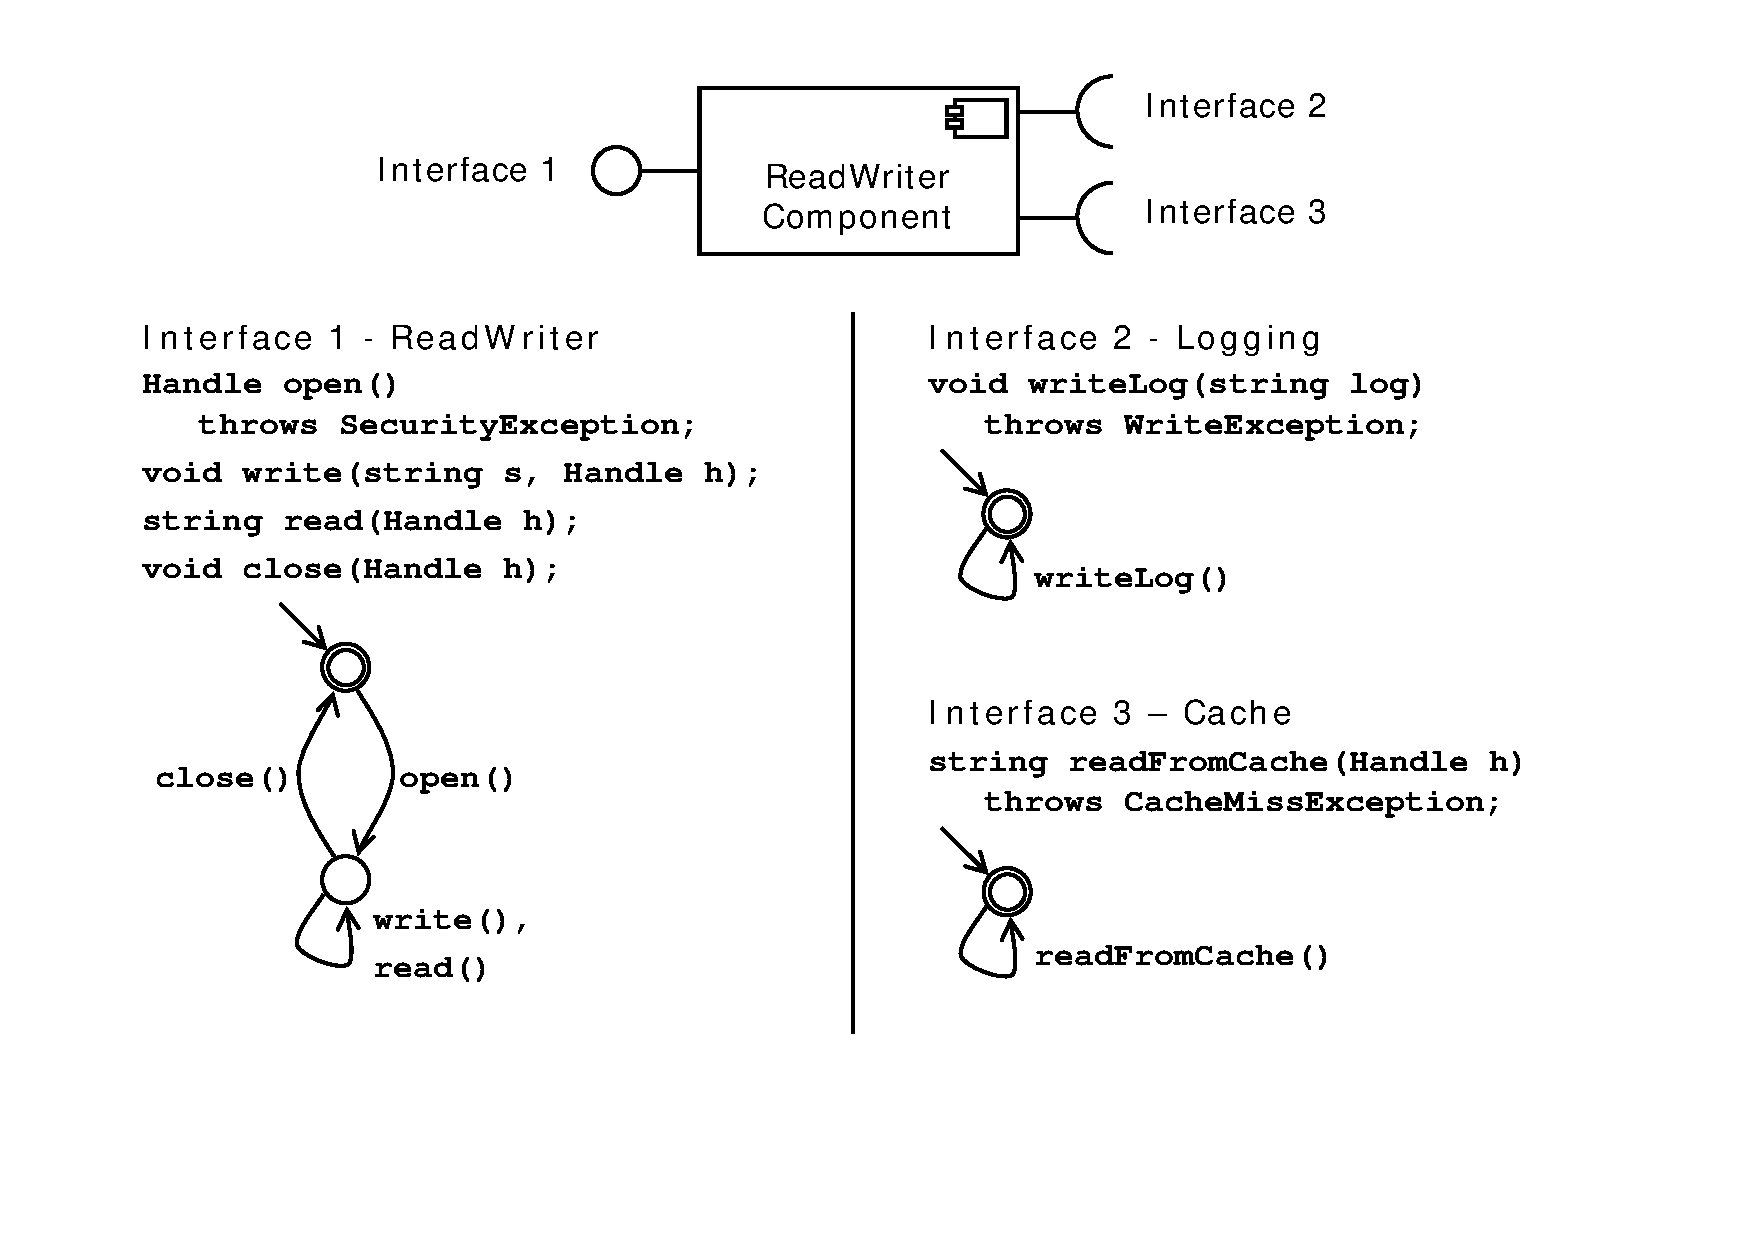
\includegraphics[width=1.00\textwidth]{./image/cm-interfaces-signature-protocol-01.pdf}
	\caption{Beispielschnittstellen mit Signaturlisten und Protokollinformationen in Form von endlichen Automaten}
	\label{fig:cm-interfaces-signature-protocol-01}
\end{figure}



Bisher wurden Schnittstelle nicht n�her charakterisiert. Daher konnten auch keine Interoperabilit�tsbedingungen f�r Komponenten definiert werden. Wesentliche Eigenschaften einer Schnittstelle werden durch die Signaturliste und durch das Protokoll bestimmt. Auf Schnittstellen k�nnen innerhalb von Signaturlisten Dienste definiert sein, sowie ein Protokoll, das g�ltige Aufrufreihenfolgen von Diensten definiert.

Abbildung \ref{fig:cm-interfaces-signature-protocol-01} zeigt eine Beispielskomponente "`ReadWriter Component"', die die Schnittstelle "`Interface 1"' anbietet und die Schnittstellen "`Interface 2"' und "`Interface 3"' ben�tigt. Diese Komponente wird auch in Kapitel \ref{sec:ServiceEffektSpezifikation} als Beispiel verwendet. Zudem wird zu jeder Schnittstelle eine beispielhafte Signaturliste mit dazu geh�rigem Protokoll im Form eines endlichen Automaten gezeigt.



\subsubsection{Signaturlisten und Signaturen}
\label{sec:SignaturlistenundSignaturen}
Jeder Dienst weist auf einer Schnittstelle eine eindeutige Signatur auf, etwa \texttt{void} \texttt{Do\-Some\-thing(int a)}. In Anlehnung an Methoden"=Signaturen aus Programmiersprachen wie C\# und Java haben Signaturen

\begin{itemize}
	\item einen R�ckgabe"=Datentyp oder \texttt{void},
	\item einen Bezeichner, �blicherweise mit einem sprechenden Namen,
	\item eine Menge von Parametern (\texttt{0..*}), die jeweils aus einem Datentyp und einem Bezeichner (innerhalb der Parameter eindeutig) bestehen. Zus�tzlich k�nnen die Modifizierer \texttt{in}, \texttt{out} und \texttt{ref} f�r Parameter in Analogie zur C\# Semantik verwendet werden. Parameter werden in Klammern angegeben und durch Kommata getrennt, Modifizierer werden den Parametern vorangestellt.
	\item Daneben m�ssen alle \textit{Exceptions} (Ausnahmen) angegeben werden, die von einer Signatur geworfen werden k�nnen. Die verpflichtende Angabe von \textit{Exceptions} folgt den Vorgaben von Java. \textit{Exceptions} werden mit dem Schl�sselwort \texttt{throws} an die Methoden"=Signatur angeh�ngt und durch Kommata getrennt.
\end{itemize}

Eine Signatur ist eindeutig �ber R�ckgabe"=Datentyp, Bezeichner und Parameter (Datentyp und Bezeichner) unter Ber�cksichtigung der Reihenfolge.



Eine Schnittstelle enth�lt genau eine Signaturliste. Diese Signaturliste wiederum enth�lt \texttt{0..*} Signaturen. Signaturen und Signaturlisten k�nnen nicht zur gleichen Zeit von verschiedenen Schnittstellen referenziert werden. Gleichwohl k�nnen verschiedene Schnittstellen identische Signaturlisten oder einzelne Signaturen definieren. 



\subsubsection{Protokolle}
\label{sec:Protokolle}
Wie bereits oben angedeutet, definieren Protokolle von Schnittstellen g�ltige Aufrufsequenzen auf Diensten. In Abbildung \ref{fig:cm-interfaces-signature-protocol-01} werden beispielhaft endliche Automaten zur Darstellung der Protokolle auf den Schnittstellen verwendet. Das Komponentenmodell limitiert dabei Protokolle nicht auf einen bestimmen Typ, wie endliche Automaten oder Petri"=Netze, sondern l�sst diese Entscheidung bewu�t offen. Schnittstellen m�ssen nicht zwangsl�ufig Protokolle definieren.

Um im Beispiel zu bleiben: hier beginnen alle g�ltigen Aufrufsequenzen mit einem \texttt{open()}, gefolgt von beliebigen \texttt{read()} und \texttt{write()} Operationen. In jedem Fall muss abschlie�end ein \texttt{close()} folgen. Alternativ sind auch Sequenzen g�ltig, die sofort enden (denn direkt nach dem Initialisieren befindet sich das Protokoll der Schnittstelle in einem g�ltigen Endzustand). Als Kantenbeschriftungen werden also Signaturen aus der Signaturliste der mit einem Protokoll zu versehenden Schnittstelle verwendet.

Protokolle bieten somit eine M�glichkeit Abh�ngigkeiten zwischen Diensten, respektive Signaturaufrufen, \textit{einer} Schnittstelle zu definieren. Damit wird f�r Komponenten ein interner Zustand m�glich. �ber Dienstaufrufe kann der Zustand ver�ndert werden. Abh�ngig von aktuellen Zustand sind nur bestimmte weitere Dienstaufrufe m�glich. Nur bestimmte Sequenzen, n�mlich jene, die zu einem Endzustand f�hren, sind g�ltig. Von Komponenten kann nur dann ein definiertes Verhalten erwartet werden, wenn die Schnittstellenprotokolle erf�llt werden.



\paragraph{Einschr�nkungen}
\label{sec:EinschraenkungenProtokoll}
Das Komponentenmodell erlaubt indes derzeit keinen Zustandswechsel in Abh�ngigkeit von Aufrufparametern einer Signatur. Um weitere Zustandswechsel einer Komponente modellieren zu k�nnen, ist es notwendig die Zahl der Signaturen zu erh�hen. Damit kann, bei endlichen Parameterwerten, ein Verhalten nachgebildet werden, dass einer Abh�ngigkeit des internen Komponentenzustands von Parameterwerten entspricht.

Zu beachten ist, dass Schnittstellen ein Protokoll definieren k�nnen, der Zustand jedoch von der implementierenden und anbietenden (\textit{provides}) Komponente abh�ngt.

Als weitere Einschr�nkung des Komponentenmodells gilt derzeit, dass eine Komponente mehrere Schnittstellen zugleich anbieten oder ben�tigen kann. Innerhalb der Menge der angebotenen \textit{oder} ben�tigten Schnittstellen gibt es jedoch keine M�glichkeit schnittstellen�bergreifende Protokolle zu definieren. Somit kann eine Komponente zur gleichen Zeit \textit{mehrere} interne Zustande haben. Je Schnittstellenprotokoll existiert ein eigener Zustand. Damit l�sst sich kein Verhalten modellieren, bei dem sich Schnittstellenaufrufe gegenseitig beeinflussen. Denkbar w�ren hier sich gegenseitig blockierende Aufrufe auf Grund einer gemeinsamen kritischen Ressource.



\paragraph{Schlechte Modellierung}
\label{sec:SchlechteModellierung}
Sind die Signaturlisten und Protokolle, die auf verschiedenen Schnittstelle definiert wurden, identisch, deutet dies zumeist auf ein Design"=Problem des Komponentenmodells hin. Sind auch Zusatzattribute (z. B. Quality"=of"=Service"=Attribute; siehe Kapitel ref{TODO Anotationen}) identisch, f�hrt dies vermutlich zu ungewollten Inkonsistenzen zwischen einer vermeintlich identischen Schnittstelle.



\subsection{Service Effekt Spezifikation}
\label{sec:ServiceEffektSpezifikation}



\begin{figure}[htbp]
	\centering
		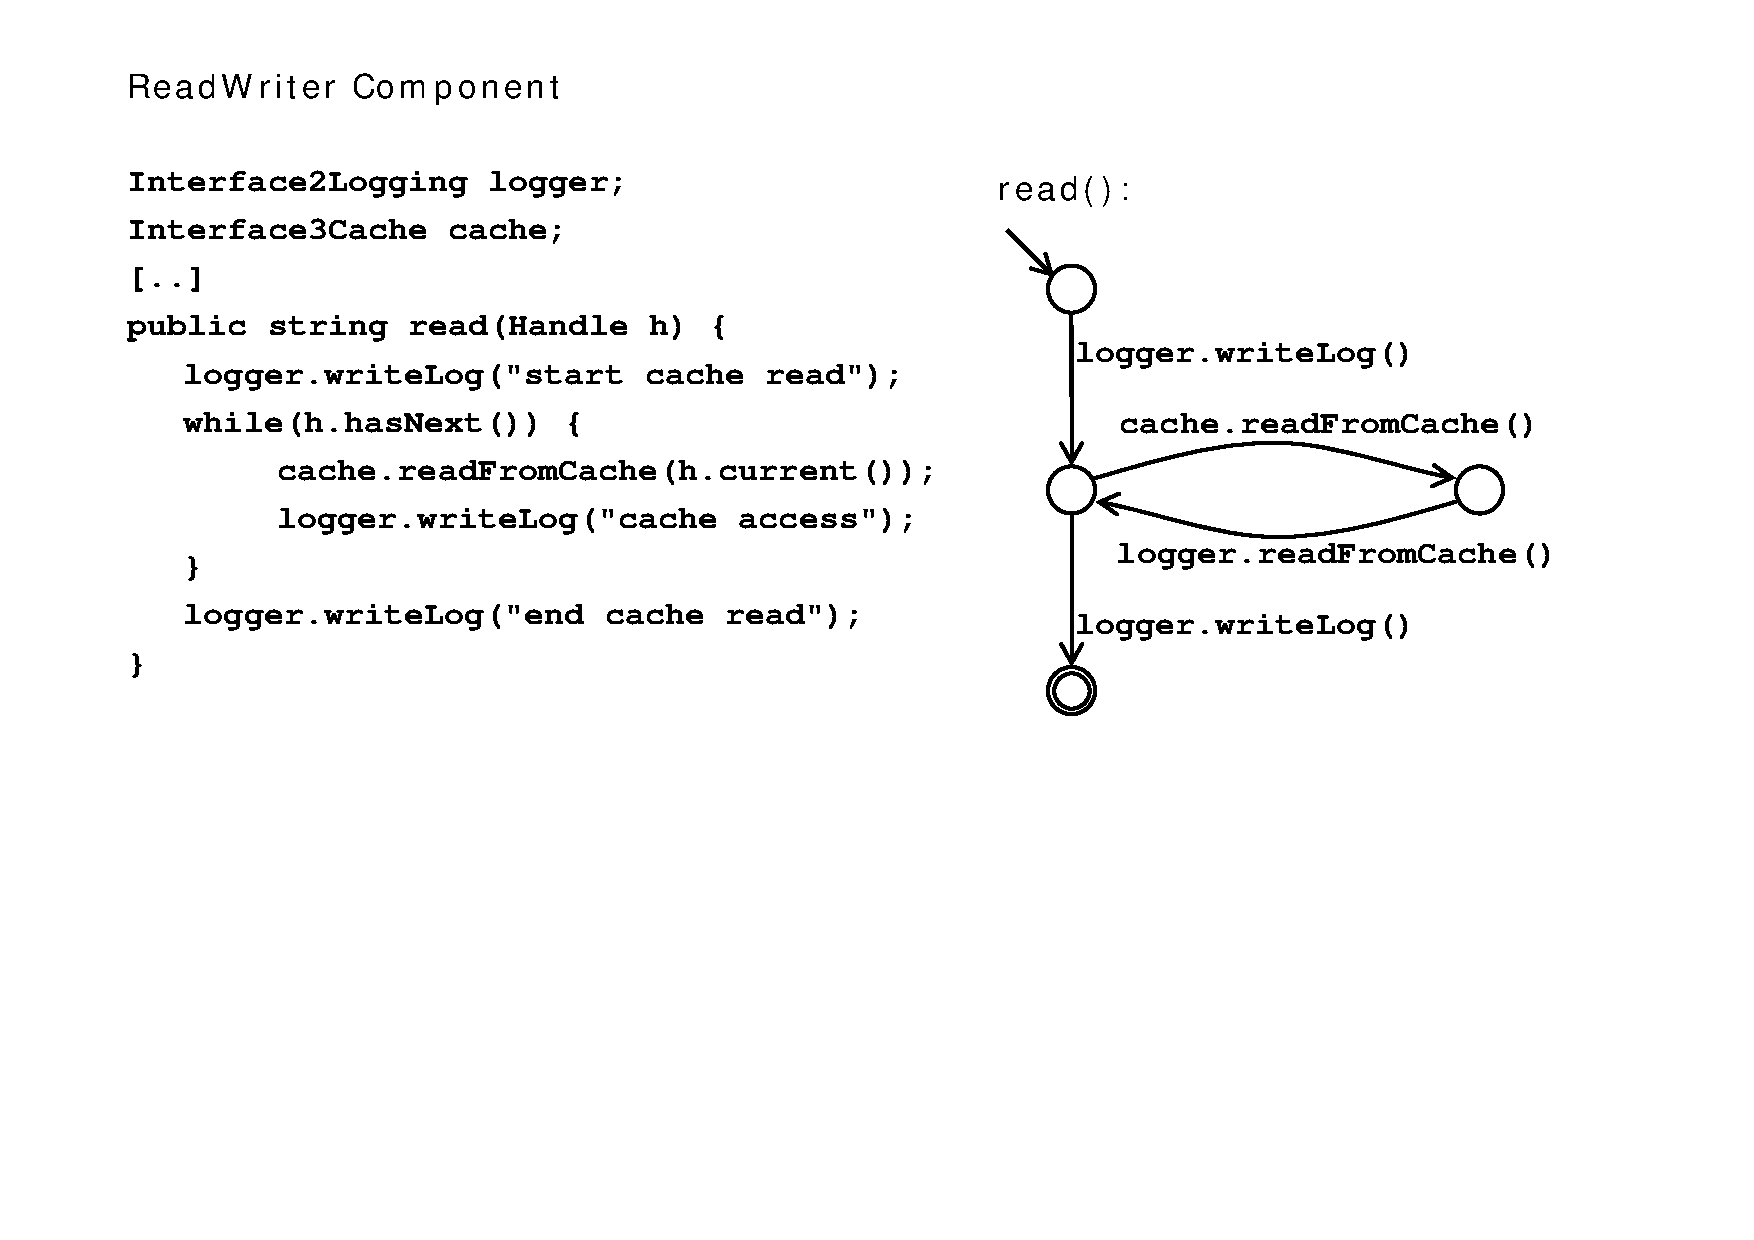
\includegraphics[width=1.00\textwidth]{./image/cm-code-seff-01.pdf}
	\caption{Service Effekt Spezifikation als endlicher Automat zu beispielhaftem Pseudo"=Quellcode}
	\label{fig:cm-code-seff-01}
\end{figure}



W�hrend Protokolle g�ltige Aufrufsequenzen auf Schnittstellen beschreiben, stellen Service Effekt Spezifikationen, auch SEFF (\textit{Service Effect Specification}), eine Verbindung zwischen angebotenen und ben�tigten Schnittstellen einer Komponente her. SEFFs sind grunds�tzlich nur f�r \textit{Basic Components} zugelassen, da nur diese Form der Komponenten eine Realisierung enth�lt, die nicht auf weitere interne Komponenten verweist.

Wie der Name andeutet, beschreibt ein SEFF zu genau einem angebotenem Dienst (\textit{Service} des \textit{Provides Interfaces}) einer Komponente die externen Auswirkungen auf die ben�tigte Schnittstelle. Interne Vorg�nge in der Komponente werden dabei abstrahiert. Daf�r werden s�mtliche Aufrufe auf externen Komponenten (�ber die ben�tigten Schnittstellen) erfasst. Damit ist es m�glich die Auswirkungen eines Dienstaufrufs auf einer Komponente "`durch die Komponente hindurch"' zu beobachten. Zus�tzlich werden Kontrollfluss"=Elemente der zu beschreibenden Komponente erfasst, sofern diese Kontrollfluss"=Elemente Auswirkungen auf die externen Aufrufe haben.

In Abbildung \ref{fig:cm-code-seff-01} wird eine Service Effekt Spezifikation zu der in Abbildung \ref{fig:cm-interfaces-signature-protocol-01} eingef�hrten Komponente dargestellt. In diesem Beispiel wird wiederum auf endliche Automaten (\textit{Finite State Machine}, FSM) zur Darstellung von SEFFs zur�ckgegriffen. Auch an dieser Stelle limitiert das Komponentenmodell nicht auf die Verwendung von endlichen Automaten. Ebenso sind Petri"=Netze oder andere Sprachen m�glich. Die m�glichen Typen von SEFFs m�ssen die SEFF"=Anforderungen spezialieren, also einen Sub"=Typ der SEFF"=Anforderungen bilden. Somit sind endliche Automaten, sofern sie im Komponentenmodell verwendet werden, eine Spezialisierung von SEFFs. Damit einher geht die Forderung, dass es eine Abbildungsvorschriften zur bijektiven Abbildung zwischen SEFF und endlichem Automaten gibt.

Da die Verwendungsreihenfolge von geforderten Diensten auch vom Zustand einer Komponente oder den Aufrufparametern eines angebotenen Dienstes abh�ngen kann, werden \textit{SEFFs} beispielsweise als endliche Automaten dargestellt, damit auch Endscheidungen (beispielsweise \texttt{if}-Ausdr�cke) oder Schleifen (etwa \texttt{while}) erfasst werden k�nnen.

Im Beispiel werden alle Initialisierungsvorg�nge der Komponente (Konstruktoraufrufe, Variablen anlegen) ausgeblendet. Der erste Aufruf, der von Interesse ist, ist der Aufruf des Loggers (\texttt{logger.writeLog()}). Als n�chstes werden die Kontrollfluss"=Elemente der Komponente abgebildet. Da \texttt{cache.readFromCache()} und \texttt{logger.writeLog()} in einer \texttt{while}"=Schleife aufgerufen werden k�nnen, wird ein Zwischenzustand eingef�hrt, der den Zustand nach dem Aufruf des Cache"=Zugriffs repr�sentiert und ein Kante, die zum Zustand vor / nach der \texttt{while}"=Schleife zur�ck f�hrt.

Bei SEFFs werden die Kanten eines endlichen Automaten mit den externen Dienstaufrufen beschriftet. Die Zust�nde des Automaten repr�sentieren den "`Zustandsbereich"' der Komponente zwischen den externen Aufrufen.



\paragraph{SEFF-Typen}
\label{sec:SEFF-Typen}
F�r jeden Dienst einer Komponente k�nnen \texttt{0..1} SEFFs eines SEFF"=Typs definiert werden. Als SEFF"=Typ gelten dabei endliche Automaten, Petri"=Netze und sonstige Sprachen (TODO: spracherzeugenden konstrukte). Existieren zu einem Dienst einer Komponent SEFF"=Beschreibungen unterschiedlichen Typs, so m�ssen diese konsistent sein, d�rfen sich also nicht widersprechen. Das Komponentenmodell pr�ft zun�chst in keinem Fall auf diese Konsistenz. Entsprechende Pr�fungen m�ssen durch den Nutzer erfolgen (Eine Pr�fung ist nicht in jedem Fall trivial: "`Sprachinklusion... TODO"'). 

Das Komponentenmodell verzichtet bewu�t auf die Einschr�nkung nur einen SEFF"=Typ global im gleichen Komponentenmodell oder f�r einen Dienst zuzulassen. Dies erlaubt es die gleiche Komponentenarchitektur zur gleichen Zeit auf verschiedene Weise mit Informationen anzureichen. Dadurch k�nnen Modellierer, auch ohne Kenntnis von der spezifischen Darstellung von SEFFs, ihre eigenen Darstellungsformen verwenden. Im Sinne der Unabh�ngigkeit des Komponentenmodells von konkreten SEFF"=Typen, bleibt es durch dieses Weniger an Einschr�nkung m�glich das Komponentenmodell gefiltert zu betrachten. Zugleich erkauft man sich diesen Vorteil durch die Gefahr, dass Inkonsistenzen verschiedener SEFF"=Typen auftreten oder spezielle SEFF"=Typen schlicht nicht verstanden werden und dadurch auch nicht konsistent zu halten sind.



\paragraph{Einschr�nkungen}
\label{sec:EinschraenkungenSEFF}
TODO: Was ist nicht mit endlichem Automaten darstellbar?



\subsection{Berechnung von SEFFs und Protokollen}
\label{sec:BerechnungvonSEFFsundProtokollen}
Eine vollst�ndige Berechnung von Protokollen und SEFFs ist nicht Gegenstand der Ausf�hrungen in dieser Diplomarbeit. Um dennoch abgrenzen zu k�nnen, welche Berechnungen grunds�tzlich m�glich sind, wird in den folgenden beiden Unterkapiteln grob dargestellt, wie die m�glichen Berechnungen durchf�hrbar sind und welche Einschr�nkungen sich dadurch f�r manuell spezifizierte SEFFs und Protokolle ergeben.



\subsubsection{Berechnung von ben�tigten Protokollen}
\label{sec:BerechnungvonbenoetigtenProtokollen}



\begin{figure}[htbp]
	\centering
		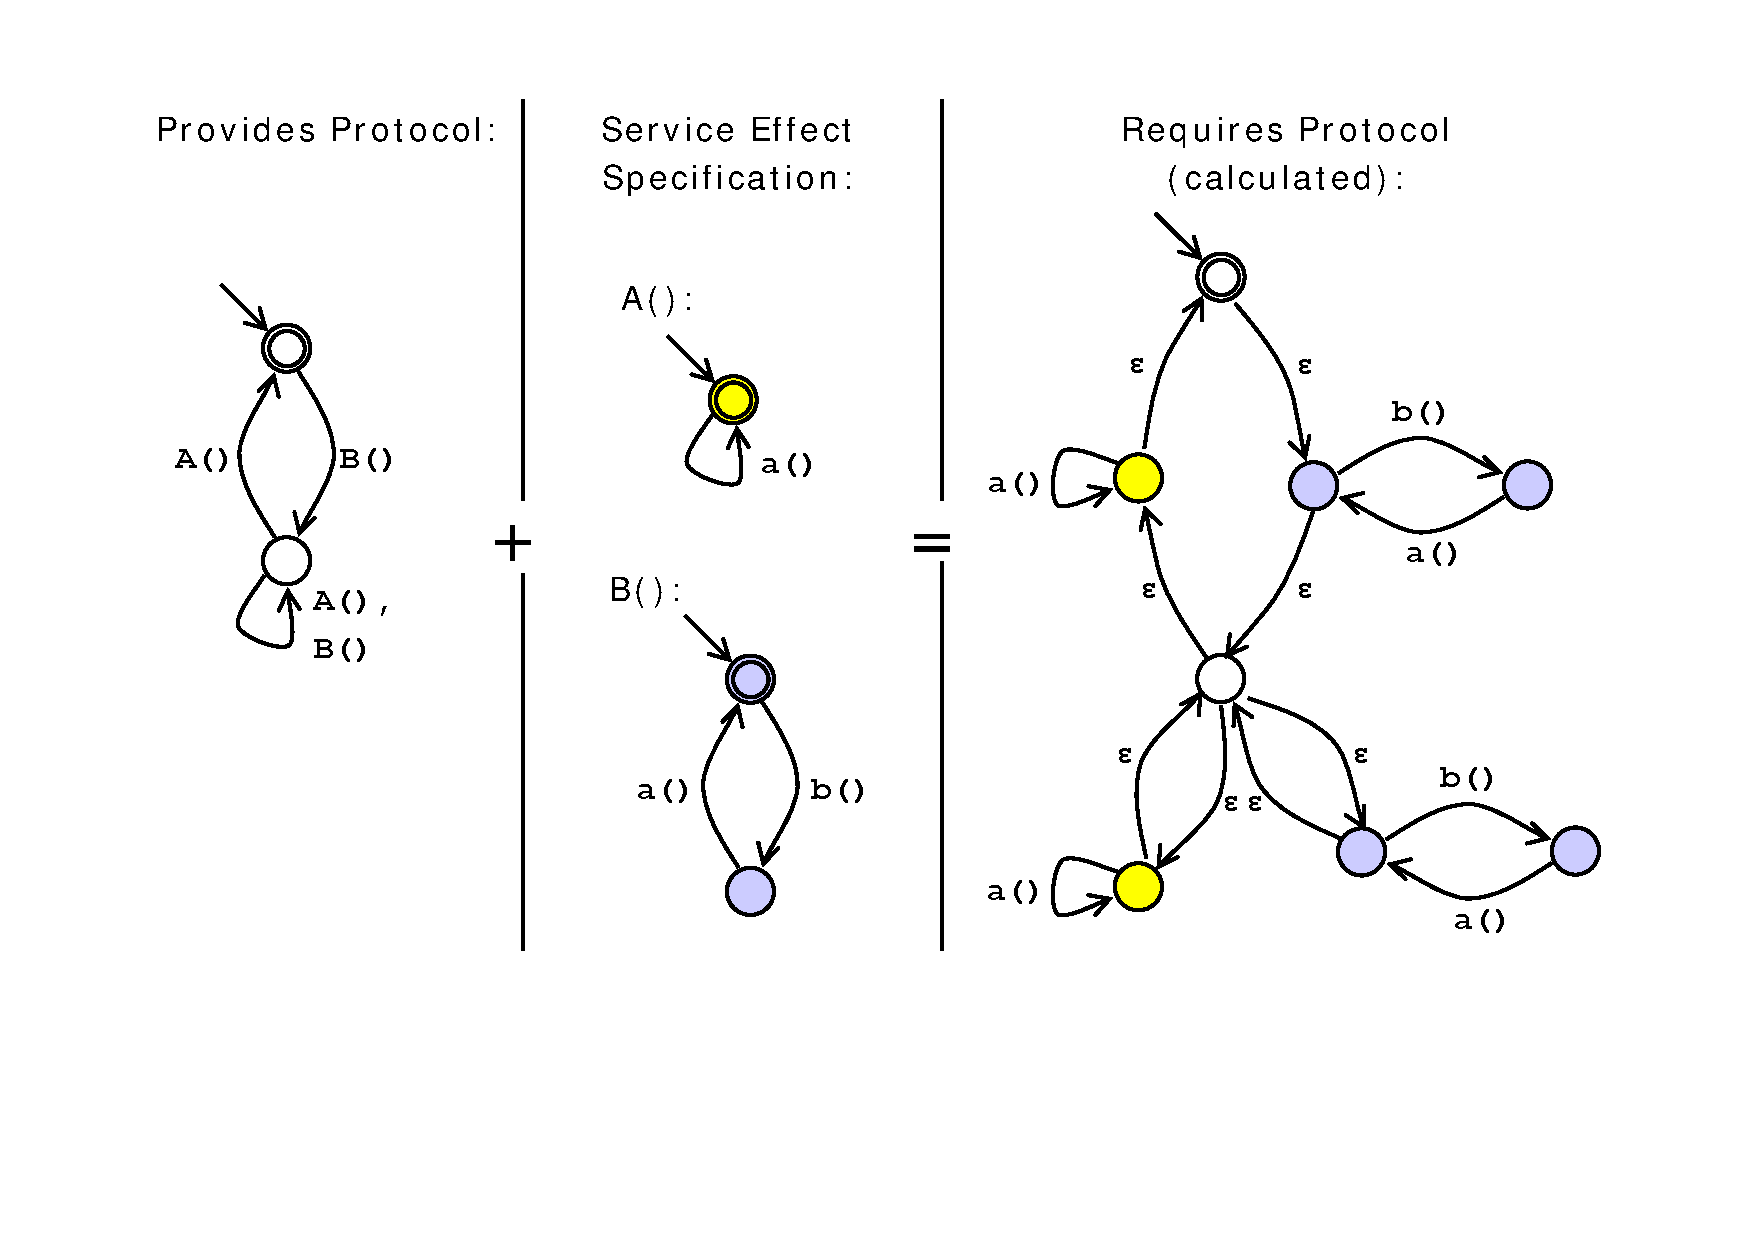
\includegraphics[width=0.80\textwidth]{./image/cm-calculated-requires-protocol-01.pdf}
	\caption{Beispiel der Berechnung eines \textit{Requires Protocols} aus einem \textit{Provides Protocol} und SEFFs}
	\label{fig:cm-calculated-requires-protocol-01}
\end{figure}



Da SEFFs eine Verbindung zwischen den Protokollen auf der angebotenen und ben�tigten Seite herstellen, l��t sich sich zu einem gegebenen angebotenem Protokoll mit Hilfe eines SEFFs ein ben�tigtes Protokoll berechnen. Abbildung \ref{fig:cm-calculated-requires-protocol-01} zeigt exemplarisch die Berechnung eines \textit{Requires Protocols} aus einem \textit{Provides Protocol} und SEFFs anhand endlicher Automaten.

Kurz skizziert erfolgt eine Erweiterung des angebotenen Protokolls. Dazu wird das angebotene Protokoll als Grundlage genommen und f�r jede Transition dieses Automaten wird der Automat des SEFFs eingef�gt, der die Realisierung der Methode aus der Beschriftung der Kante enth�lt. Die Endzust�nde des SEFFs werden dabei entfernt. Um die aus dem SEFF stammenden Teilautomaten in das urspr�ngliche angebotene Protokoll einzuf�gen, werden zwei $\epsilon$"=Transitionen eingef�gt: eine f�hrt vom urspr�nglichen Startzustand der Transition aus dem angebotenem Protokoll in den urspr�nglichen Startzustand des SEFF"=Automaten. Eine weitere $\epsilon$"=Transition f�hrt vom urspr�nglichen Endzustand des SEFF"=Automaten in den urspr�nglichen Folgezustand der ersetzten Transition des angebotenen Protokolls.

Wird dieses Prozedere f�r jede Transition des angebotenen Protokolls durchgef�hrt, erh�lt man ein ben�tigtes Protokoll der Komponente. An dieser Stelle soll nicht n�her auf die Berechnung des ben�tigten Protokolls eingegangen, sondern lediglich kurz skizziert werden, dass eine M�glichkeit besteht das ben�tigte Protokoll zu berechnen. Daraus ergibt sich die Notwendigkeit, dass, sofern ben�tigte Protokolle manuell spezifiziert werden, diese konsistent zu einer berechneten Form sein m�ssen. �blicherweise wird man jedoch auf eine manuelle Spezifikation des ben�tigten Protokolls verzichten und dieses berechnen lassen.



\subsubsection{Berechnung der SEFFs von Composite Components}
\label{sec:BerechnungderSEFFsvonCompositeComponents}



\begin{figure}[htbp]
	\centering
		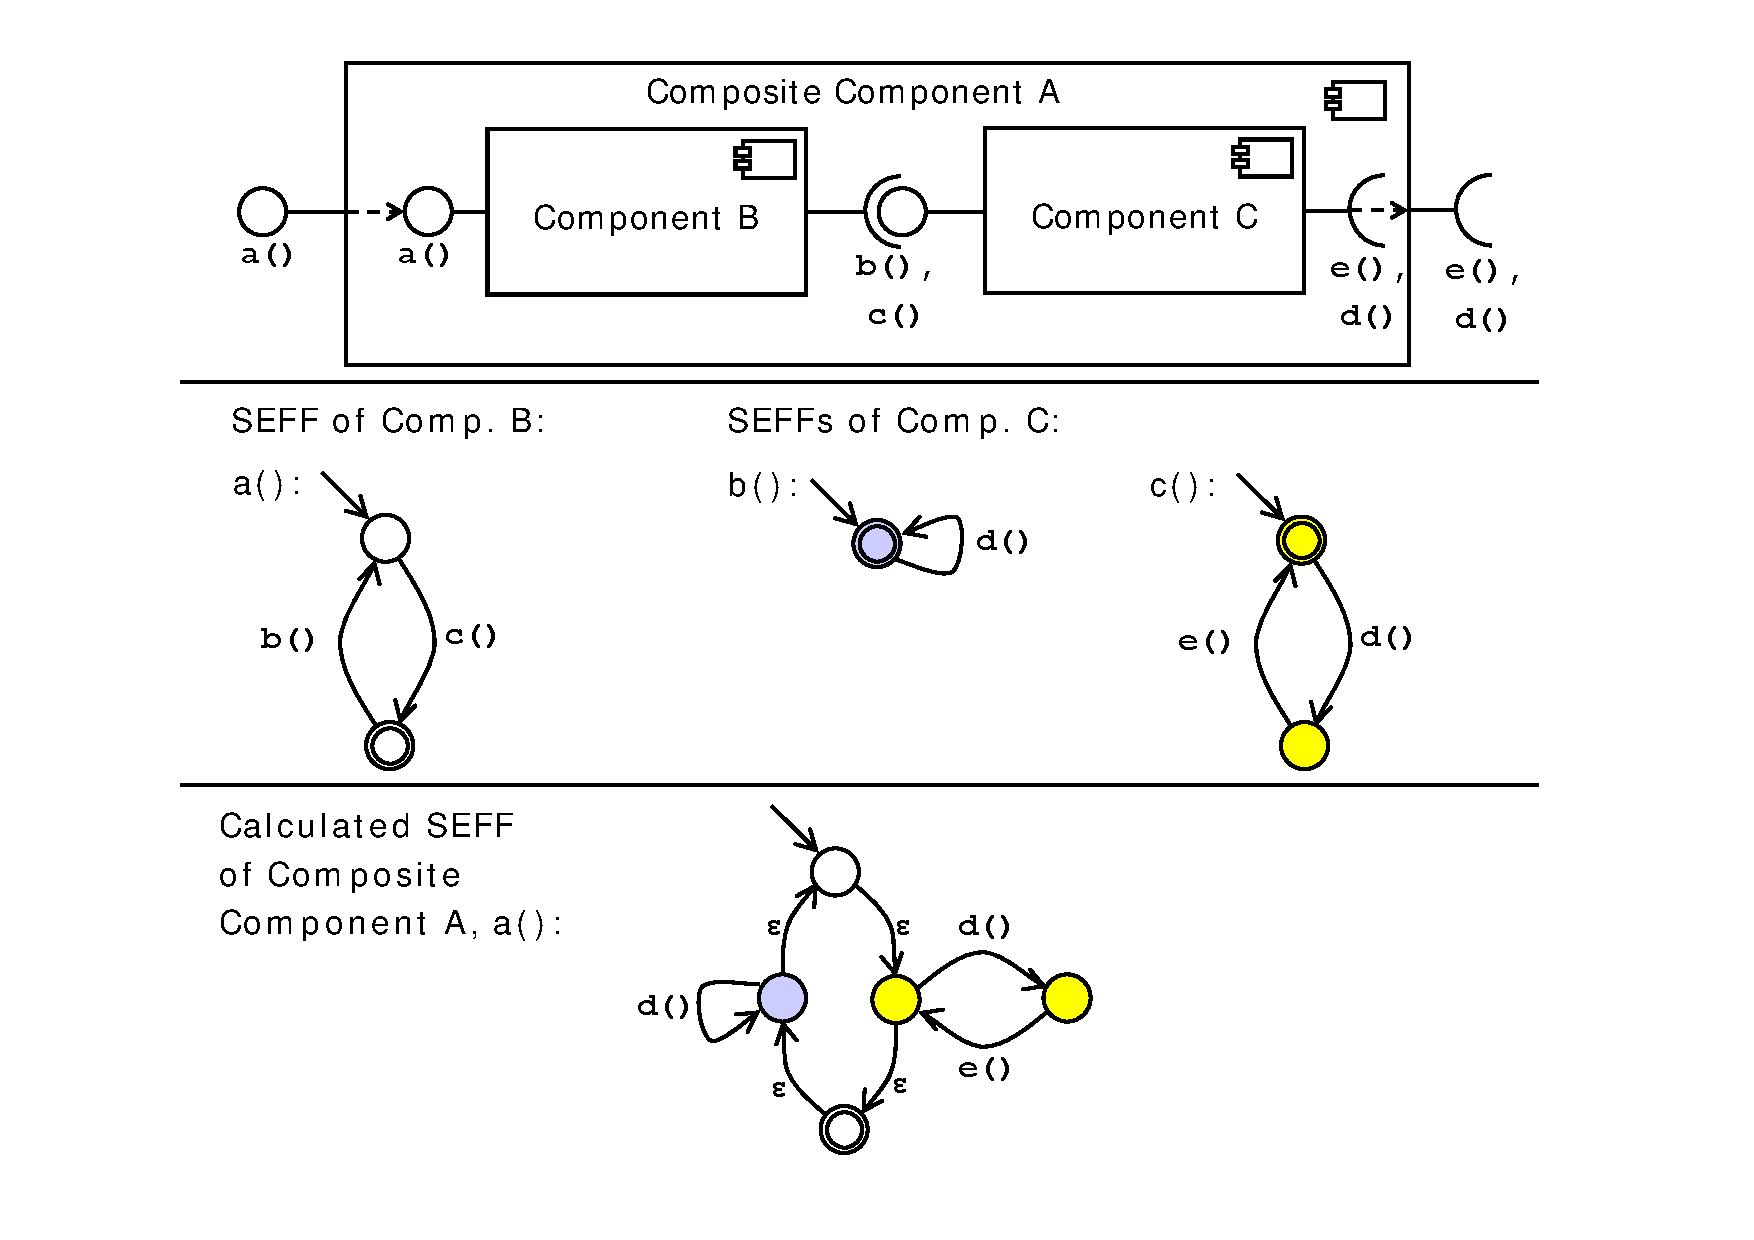
\includegraphics[width=0.80\textwidth]{./image/cm-calculated-cc-seff-01.pdf}
	\caption{Beispiel der Berechnung eines SEFFs f�r eine \textit{Composite Component} bei endlichen Automaten}
	\label{fig:cm-calculated-cc-seff-01}
\end{figure}



In Kapitel \ref{sec:ServiceEffektSpezifikation} wurde bereits dargelegt, weshalb \textit{Composite Components} selbst keine SEFFs besitzen. Dennoch l��t sich f�r \textit{Composite Components} ein SEFF berechnen. Dieser ergibt sich aus den zusammengesetzten SEFFs innenliegender Komponenten. Entsprechend ist ein solcher SEFF nur berechenbar, wenn auch f�r alle innenliegenden Komponenten, einschlie�lich innerer \textit{Composite Components}, SEFFs vorliegen. Liegen f�r alle inneren (auch rekursiv absteigend) Komponenten vollst�ndig \textit{Basic Components} und somit auch SEFFs vor, lassen sich die SEFFs h�her liegender \textit{Composite Components} rekursiv berechnen. Damit wird dann schlie�lich auch der SEFF der zu betrachtenden Composite Component berechenbar. Bei einem voll spezifizierten Modell (siehe auch Implementation"=Type in Kapitel \ref{sec:Typ-Ebenen}) verweisen letztlich alle \textit{Composite Components} auf \textit{Basic Components}.

Abbildung \ref{fig:cm-calculated-cc-seff-01} zeigt beispielshaft die Berechnung von SEFFs f�r eine \textit{Composite Component} aus den SEFFs zweier Sub"=Komponenten. Auch hier sind die SEFFs wieder als endliche Automaten dargestellt. �hnlich der Vorgehensweise bei der Berechnung des \textit{Requires Protocols} erfolgt auch hier eine Ersetzung von Transitionen. Zusammengefasst f�hren all jene Methodenaufrufe, die nicht aus einer \textit{Composite Component} heraus gehen, zur Ersetzung der Transition, die den Methodenaufruf repr�sentiert, mit dem SEFF, der dem Methodenaufruf entspricht. Ebenso wie beim Protokoll werden $\epsilon$"=Transition eingef�hrt, die in den Startzustand f�hren und vom Endzustand wieder zur�ck. Auch der Endzustand des eingef�gten SEFFs wird entfernt.

Im Beispiel bietet "`Composite Component A"' mit \texttt{a()} genau eine Methode an, die durch "`Component B"' implementiert wird. "`Component B"' delegiert die Aufrufe von \texttt{b()} und \texttt{c()} auf "`Component C"'. Diese Komponente ben�tigt die Methoden \texttt{e()} und \texttt{d()}. Da \texttt{e()} und \texttt{d()} nicht von einer inneren Komponente angeboten werden, f�hren diese Methodenaufrufe aus "`Composite Component A"' heraus. Zus�tzlich sind die SEFFs zu den Methodenaufrufen \texttt{a()}, \texttt{b()} und \texttt{c()} angegeben, also jene Methoden, die durch innere Komponenten angeboten werden.

Der berechnete SEFF f�r "`Composite Component A"' und die Methode \texttt{a()} ergibt sich, entsprechend dem oben skizzierten Verfahren, zun�chst aus dem SEFF f�r \texttt{a()} aus "`Component B"'. In diesem SEFF werden die Aufrufe von \texttt{b()} und \texttt{c()} durch die entsprechenden SEFFs aus "`Component C"' ersetzt (dunkelgrau bzw. blau eingef�rbte Zust�nde resultieren aus dem SEFF von \texttt{b()}; hellgrau bzw. gelb eingef�rbte Zust�nde resultieren aus dem SEFF von \texttt{c()}).

Da die Berechnung von SEFFs f�r \textit{Composite Components} damit problemlos und effizient m�glich ist, unterst�tzt das Komponentenmodell f�r zusammengesetzte Komponenten nur berechnete SEFFs. Diese haben den Vorteil automatisch konsistent mit den inneren SEFFs einer Komponente gehalten werden zu k�nnen.



\subsection{Komponenten: Typ-Ebenen}
\label{sec:Typ-Ebenen}
Das Palladio Komponentenmodell umfasst das Konzept verschiedener Modellierungs"=Ebenen f�r eine Modell"=Auspr�gung. Die Modellierungs"=Ebenen spiegeln sich dabei in Ebenen eines sich detaillierenden Typ"=Begriffs f�r Komponenten wider. Dies bedeutet, dass es m�glich ist, auf verschiedenen Abstraktionsniveaus eine Komponentearchitektur zu modellieren. Damit wird ein \textit{Top"=Down}"=Vorgehen (vgl. \cite{WikiTopDown}) bei der Modellierung gesondert unterst�tzt. Es ist m�glich gezielt Komponentendetails hinzuzuf�gen. Dabei werden f�r die Detaillierung durch das Komponentenmodell \textit{Conforms}-Beziehungen definiert, denen die Verfeinerung folgen muss. Somit lassen sich Verfeinerungen konsistent �ber Typ"=Ebenen hinweg durchf�hren.

Da das Komponentenmodell zur gleichen Zeit Komponenten verschiedener Typ"=Ebenen -- auch Typ"=Niveaus genannt -- in einem Modell unterst�tzt, sind auch auch gemischte Vorgehen aus \textit{Top"=Down} und \textit{Bottom"=Up} "`Gegenstrom"' m�glich. Detailinformationen k�nnen somit auch nur jenen Komponenten hinzugef�gt werden,

\begin{itemize}
	\item die aktuell von Interesse sind,
	\item die bei iterativem Vorgehen bereits behandelt wurden,
	\item �ber die �berhaupt Detailinformationen vorliegen,
	\item die die Informations"=Komplexit�t nicht sprengen und unter Umst�nden die Berechenbarkeit einer Modellinstanz erhalten.
\end{itemize}

Anders herum k�nnen Komponenten, deren Detail"=Beschreibung man beispielsweise �ber Reflection"=Mechanismen (vgl. \cite{DotNetComponents}, S. 412ff f�r .NET) gewonnen hat, abstrahiert in das Komponentenmodell �bernommen werden.



\subsubsection{Typ-Hierarchie}
\label{sec:Typ-Hierarchie}



\begin{figure}[htbp]
	\centering
		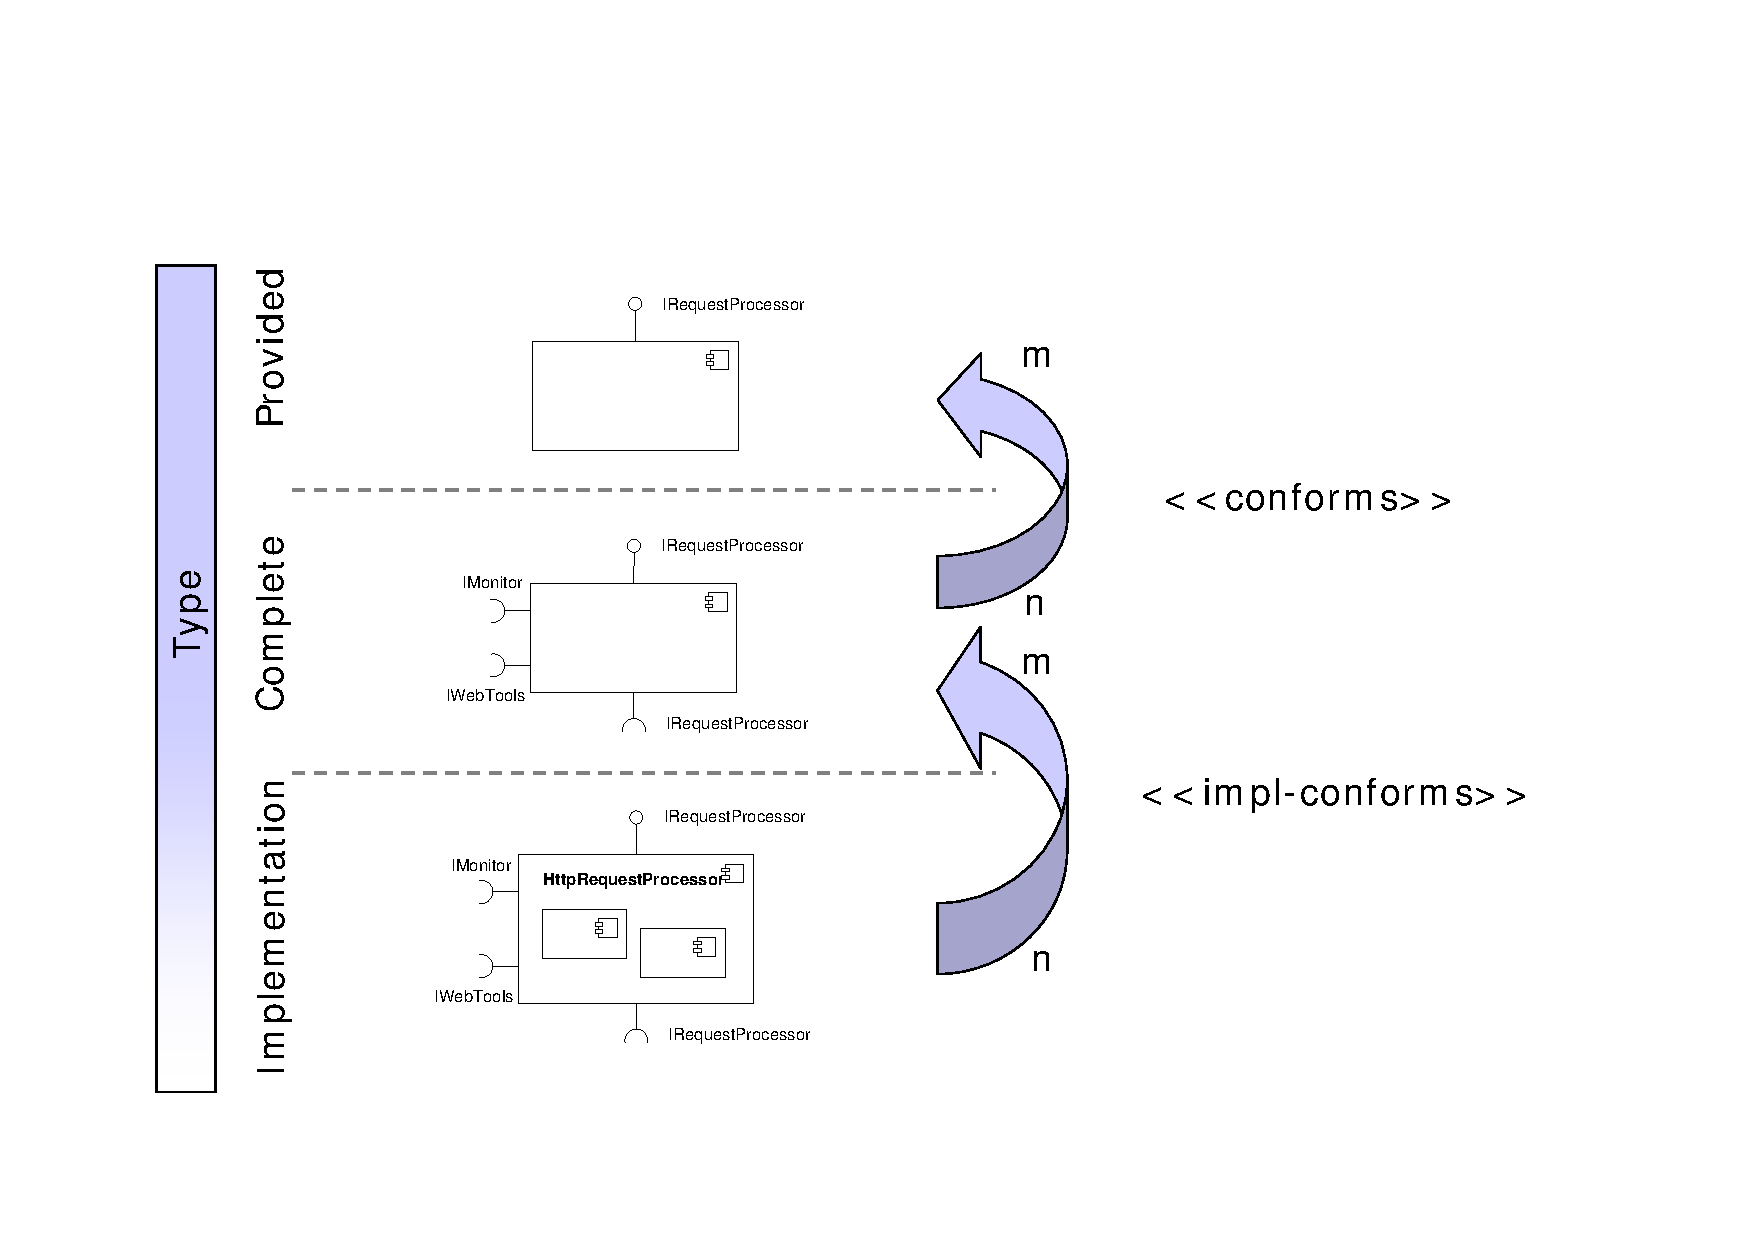
\includegraphics[width=1.00\textwidth]{./image/cm-type-levels-01.pdf}
	\caption{Typ-Hierarchie: \textit{Provided Type}, \textit{Complete Type} und \textit{Implementation Type} (nach \cite{PalladioCMNeuSlides}, S. 18)}
	\label{fig:cm-type-levels-01}
\end{figure}



Im Komponentenmodell wird derzeit in drei Typ"=Ebenen f�r Komponenten unterschieden, die einander in der angegebenen Reihenfolge nach unten spezialisieren:

\begin{itemize}
	\item \textit{Provided Type}
	\item \textit{Complete Type}
	\item \textit{Implementation Type}
\end{itemize}

In Abbildung \ref{fig:cm-type-levels-01} wird die Typ"=Hierarchie des Komponentenmodells dargestellt. Zwischen den Typ"=Ebenen besteht eine \textit{Conforms}"=Beziehung, wobei sich diese zwischen (\textit{Provided Type} und \textit{Complete Type}) und (\textit{Complete Type} und \textit{Implementation Type}) unterscheidet. Zur \textit{Conform}s"=Beziehung siehe auch Kapitel \ref{sec:Typ-Spezialisierung}.

Die farbliche Hinterlegung des "`Typ"=Balkens"' auf der linken Seite deutet an, dass der \textit{Provided Type} dem "`klassischen"' Typ"=Verst�ndnis (vgl. \cite{CZ-SOFA-CM-Hierarchy2,CZ-SOFA-CM-Hierarchy}) entspricht, indem die angebotene Schnittstelle definiert wird, wohingegen der \textit{Implementation Type} auch Vorgaben f�r die Realisierung eines Typs macht. Letzteres wird klassischerweise weniger als Typ angesehen.

W�rde man die Typ"=Hierarchie nach unten weiter f�hren, d�rfte sich noch ein Laufzeit"=Typ anschlie�en, der die Laufzeiteigenschaften einer Komponente reglementiert. Diese Typ"=Ebene wird im Komponentenmodell jedoch nicht betrachtet.



\paragraph{Sub-Typ und Implementierung}
\label{sec:Sub-TypundImplementierung}
Im Folgenden werden die Begriffe Sub"=Typ und Implementierung verwendet. Zur Kl�rung der Begriffe:
\begin{itemize}
	\item \textbf{Sub-Typ.} Beim Sub"=Typ handelt es sich um eine Relation zwischen zwei Komponenten. Gilt diese Relation, so kann ein Sub"=Typ f�r den "`Ober"=Typ"' verwendet werden. Damit ist der Sub"=Typ eine Spezialisierung des "`Ober"=Typs"'. Siehe hierzu auch Kapitel \ref{sec:Typ-Spezialisierung} auf Seite \pageref{sec:Typ-Spezialisierung}. Dort wird ebenfalls auf Co- und Contra-Varianz im Zusammenhang mit Komponenten eingegangen.
	\item \textbf{Implementierung.} Wird der Begriff Implementierung verwendet, so ist im Folgenden eine Bin�rinstanz einer Komponente oder eine programmiersprachliche Repr�sentation einer Komponente gemeint. Wie im Bereich der objektorientierten Programmierung (siehe etwas \cite{visual-csharp-oop}, S. 203ff) gibt es von Komponenten"="'Vorlagen"' Implementierungen -- analog zu OO-\textit{Interfaces} und Klassen. Pr�zise betrachtet kann es zu einer Auspr�gung eines Komponenten"=Typs \texttt{0..*} Implementierungen geben.
\end{itemize}

Im Komponentenmodell wird die Laufzeitinstanz einer Komponente zun�chst nicht betrachtet.



\paragraph{Provided Type}
\label{sec:ProvidedType}
Der \textit{Provided Type} definiert nur seine angebotenen Schnittstellen. Er enth�lt keine Informationen �ber die interne Realisierung, darf diese Informationen also nicht spezifizieren. Zudem darf er keine ben�tigten Schnittstellen angeben. Dies bedeutet, dass alle Sub"=Typen und Implementierungen eines konkreten \textit{Provided Type} in der internen Realisierung frei sind und ebenfalls keine Vorgaben �ber die ben�tigten Schnittstellen einhalten muss. Damit ist der \textit{Provided Type} der Typ, der f�r Sub"=Typen und Implementierungen am wenigstens Anforderungen definiert. Auf diese Weise werden Komponenten definiert, deren Verwendungsm�glichkeiten im Vordergrund steht.

In Abbildung \ref{fig:cm-type-levels-01} wird der \textit{Provided Type} als oberste Ebene dargestellt.



\paragraph{Complete Type}
\label{sec:CompleteType}
In Erweiterung des \textit{Provided Type} erm�glicht der \textit{Complete Type} zus�tzlich die Definition der ben�tigten Schnittstellen. Ein \textit{Complete Type} muss \textit{alle} erlaubten ben�tigten Schnittstellen definieren. Dies bedeutet, dass weder Sub"=Typen noch Implementierungen mehr Schnittstellen fordern d�rfen, als im spezifiziert, zugleich aber auch nicht weniger Schnittstellen anbieten d�rfen, als �ber den \textit{Complete Type} angegeben. Wie auch der \textit{Provided Type} darf der \textit{Complete Type} keine Informationen oder Vorgaben �ber die interne Realisierung enthalten. Auch hier sind die Sub"=Typen und Implementierungen in der Umsetzung frei. Erst eine \textit{Complete Type} Komponente kann zuverl�sslich durch eine andere Komponente substituiert werden, da erst mit diesem Detailniveau die Anforderungen vollst�ndig bekannt sind (TODO: richtig?).

In Abbildung \ref{fig:cm-type-levels-01} wird der \textit{Complete Type} als mittlere Ebene dargestellt.



\paragraph{Implementation Type}
\label{sec:ImplementationType}
Neben den Anforderungen, die ein \textit{Complete Type} erf�llen muss, muss der \textit{Implementation Type} seine interne Realisierung festlegen. Das bedeutet, dass alle internen Komponenten, die direkt in einer derart typisierten Komponente enthalten sind, mit samt der assoziierten Assembly Konnektoren und Delegationskonnektoren definiert werden m�ssen.

Gegen�ber seinem \textit{Complete Type} Vater darf ein \textit{Implementation Type} weder \textit{Provides} noch \textit{Requires} Schnittstellen hinzuf�gen oder entfernen. TODO: richtig?

F�r einen \textit{Implementation Type} muss ein SEFF verpflichtend definiert werden. Im Falle von \textit{Composite Components} ist der SEFF, wie in Kapitel \ref{sec:BerechnungderSEFFsvonCompositeComponents} dargestellt, berechnet. Da sich durch die M�glichkeit und Pflicht zur Spezifikation von SEFFs das \textit{Requires Protocol} berechnet werden kann, muss dieses auch nach der Modellierung von Komponenten auf der Implementierungs"=Typ"=Ebene konsistent zwischen den Typ"=Ebenen bleiben.

Interpretiert man die akzeptierten W�rter eines SEFFs als Sprache, muss diese Sprache gr��er oder gleich der real von einer Implementierung einer Komponente akzeptierten Sprache sein. Ein SEFFs muss also eine Obermenge ($SEFF-Sprache \supseteq Implementierungssprache$) aller g�ltigen Aufrufe auf der ben�tigten Schnittstelle darstellen. Einer Implementierung einer Komponente bleibt es damit frei gestellt, ob sie beispielsweise die M�glichkeit nutzt eine Schleife unendlich oft zu durchlaufen oder nur eingeschr�nkt oft.

In Abbildung \ref{fig:cm-type-levels-01} wird der \textit{Implementation Type} als unterste Ebene dargestellt.



\paragraph{Bemerkungen}
\label{sec:BemerkungenKomponentenTyp}



\textit{Composite Components} k�nnen zur gleichen Zeit beliebige Komponententypen in ihrem Inneren vereinen, sich also intern aus unterschiedlich detaillierten Komponenten zusammensetzen.

Sowohl \textit{Composite Components} als auch \textit{Basic Components} sind \textit{Implementation Types}. Sie erben direkt von der Meta-Klasse "`Implementation Type"', wie sie in Abbildung \ref{fig:cm-component-types-inheritance-conforms-01} dargestellt wird.



\subsubsection{Darstellung und Ebenenbeziehungen}
\label{sec:DarstellungundEbenenbeziehungen}



\begin{figure}[htbp]
	\centering
		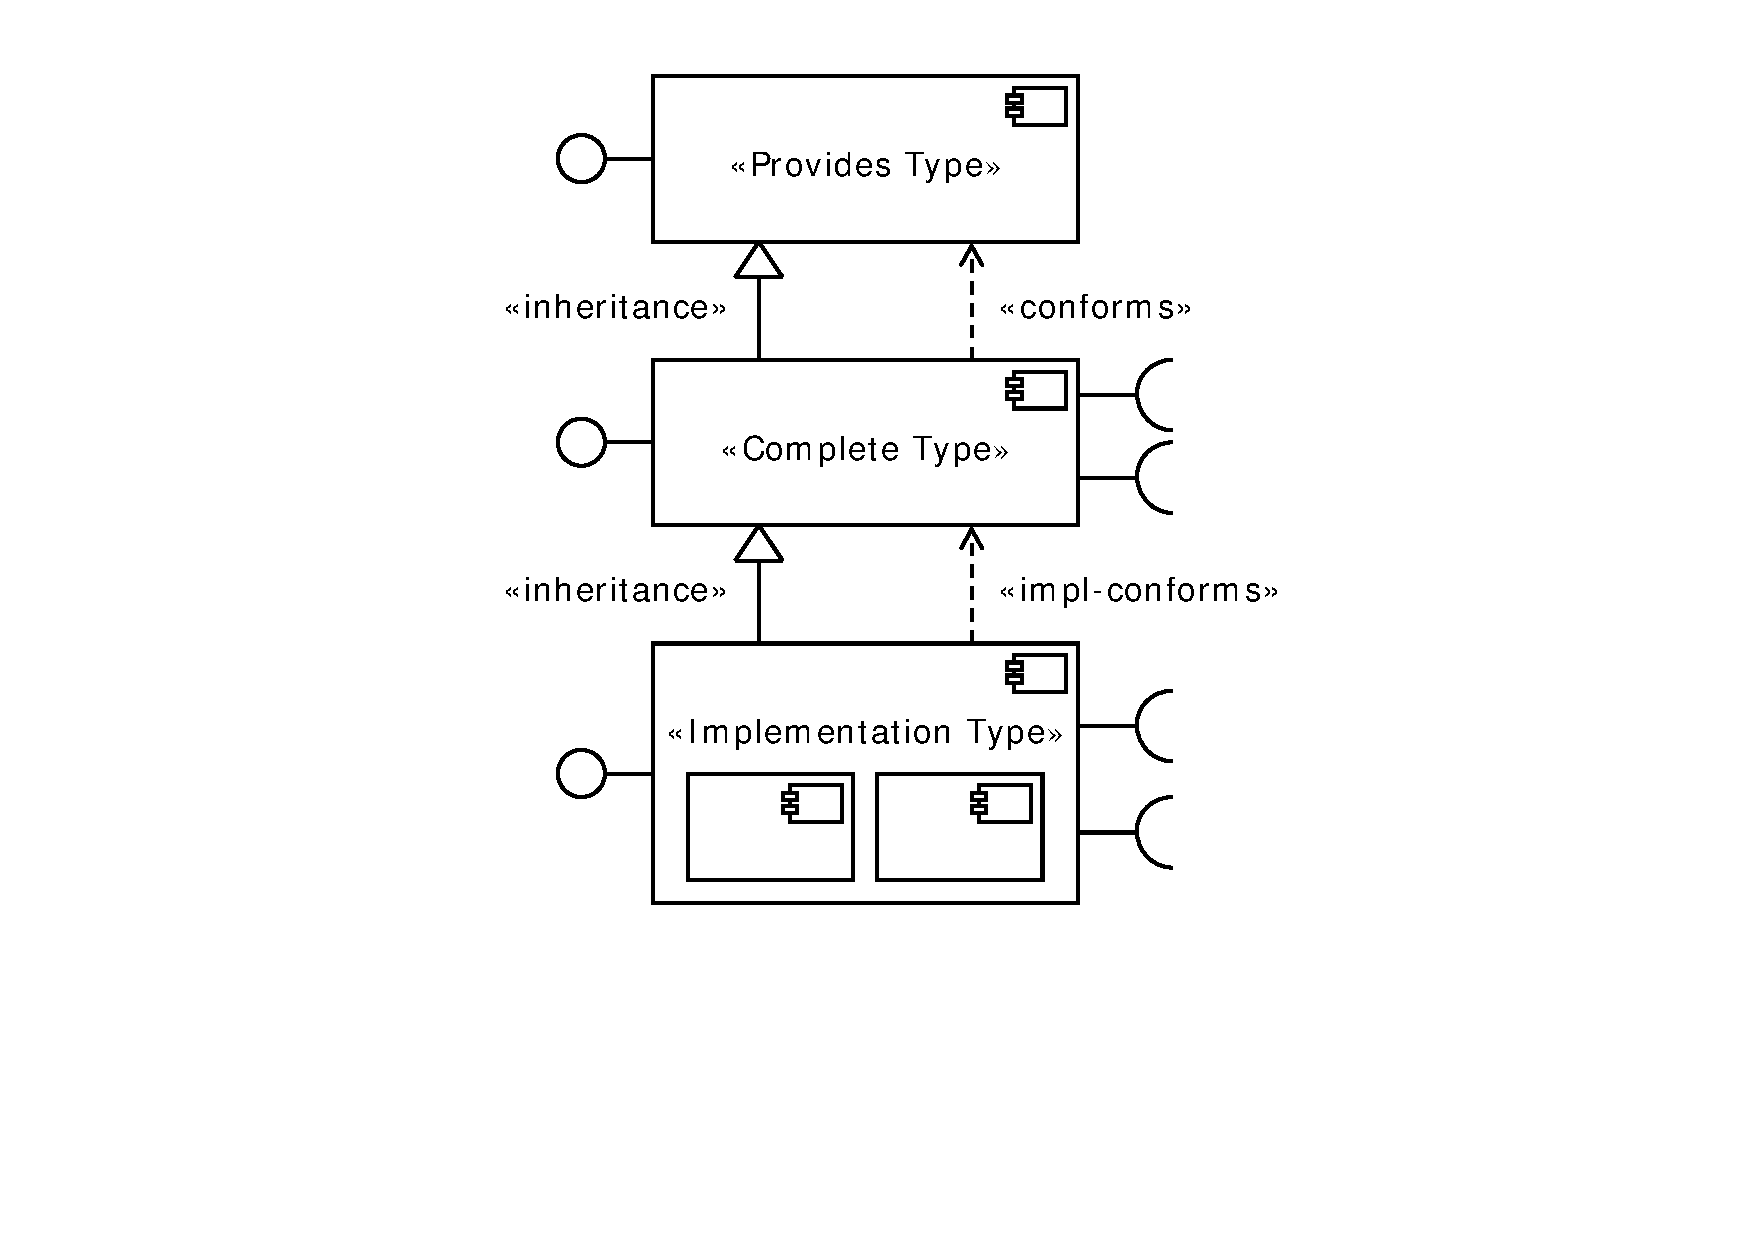
\includegraphics[width=0.50\textwidth]{./image/cm-component-types-inheritance-conforms-01.pdf}
	\caption{Komponenten Typ-Ebenen: Vererbungs- und Konformit�tsbeziehungen}
	\label{fig:cm-component-types-inheritance-conforms-01}
\end{figure}



Wie Abbildung \ref{fig:cm-component-types-inheritance-conforms-01} aufzeigt, bestehen zwischen den Typ"=Ebenen der Komponenten des Komponentenmodells paarweise jeweils zwei Beziehungen: Zum einen erben die Komponenten"=Typen jeweils von ihrem Vater"=Typ, sofern vorhanden, zum anderen erf�llen die Komponenten jeweils eine Konformit�tsbeziehung (\textit{conforms}). Das bedeutet, dass die Eigenschaften und der Informationsgehalt der Komponententypen sich ebenfalls nach unten vererben. Weiter unten stehende Komponenten"=Typen enthalten also immer mehr Informationen. Gleichzeitig bedeutet die Konformit�tsbeziehung, dass Auspr�gungen von Komponenten"=Typen, die Sub"=Typen von einander sind, festen Regeln folgen m�ssen. Somit bezieht sich die Konformit�t auf konkrete Auspr�gungen von Komponenten untereinander, wohingegen die Vererbung die Eigenschaften der Komponenten"=Typen definiert.

Die Darstellungsweise von der Typ"=Ebenen der Komponenten sollte, wie in Abbildung \ref{fig:cm-component-types-inheritance-conforms-01} angegeben, die Typ"=Ebene als Stereotyp tragen. Naheliegend f�hren \textit{Provides Types} keine ben�tigten Schnittstellen auf und \textit{Implementation Types} geben in ihrem Innern ihre Realisierung an. Anders als in der Abbildung, werden die internen Konnektoren und Schnittstellen dabei angegeben.



\subsubsection{Quantitt�ten der Sub-Typ-Beziehungen}
\label{sec:QuantittaetenderSub-Typ-Beziehungen}



\begin{figure}[htbp]
	\centering
		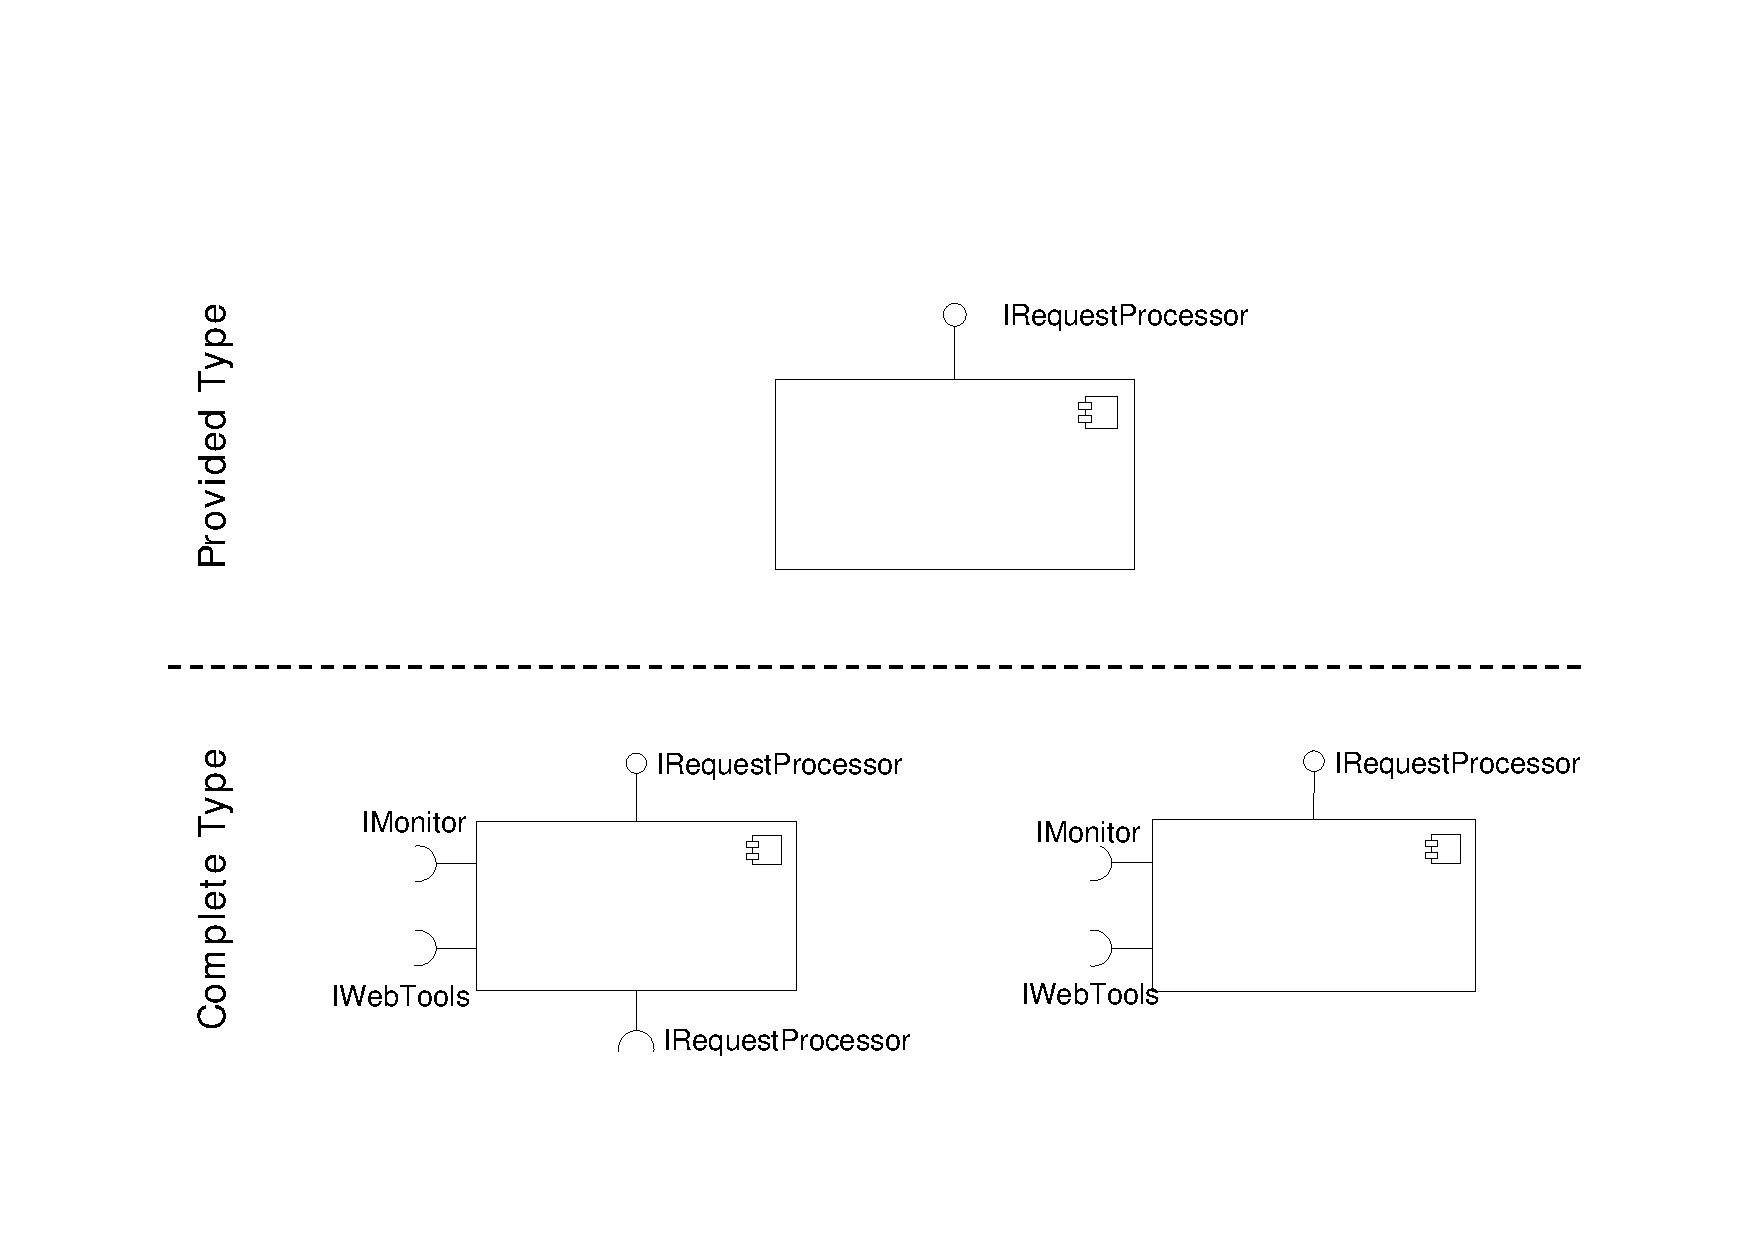
\includegraphics[width=0.80\textwidth]{./image/cm-level-refinement-01.pdf}
	\caption{Spezialisierung eines \textit{Provided Type} zu zwei \textit{Complete Types} (nach \cite{PalladioCMNeuSlides}, S. 17)}
	\label{fig:cm-level-refinement-01}
\end{figure}



\paragraph{1:n}
Zun�chst einmal soll anhand von Abbildung \ref{fig:cm-level-refinement-01} illustriert werden, dass es zu einem \textit{Provided Type} eine beliebige Menge (\texttt{0..*}) von \textit{Complete Types} geben kann. Solange das/die durch den \textit{Provides Type} vorgegebene(n) angebotene(n) Interface(s) (im Beispiel \texttt{IRequestProcessor}) vom \textit{Complete Type} angeboten wird/werden, handelt es sich um Sub"=Typen. Sub"=Typen folgen der \textit{conforms}"=Beziehung (siehe Abb. \ref{fig:cm-type-levels-01}) zwischen den betroffenen Typ"=Ebenen f�r Komponenten. Der \textit{Complete Type} kann so, wie im Beispiel mit \texttt{IMyService}, zus�tzliche Schnittstellen anbieten. Au�erdem sind die \textit{Complete Types} komplett bez�glich der ben�tigten Schnittstellen frei. Im Beispiel wird die Schnittstelle \texttt{IRequestProcessor} lediglich von der linken Komponente angeboten. Auch die im Beispiel �berschneidend angef�hrten Schnittstellen \texttt{IMonitor} und \texttt{IWebTools} sind nicht zwischen zwei Sub"=Typen des gleichen \textit{Provided Types} erforderlich .



\paragraph{m:1}
Abbildung \ref{fig:cm-type-levels-01} zeigt eine weitere Besonderheit zwischen den Typ"=Ebenen auf. Ein \textit{Complete Type} kann der Sub"=Typ einer beliebigen Anzahl (0..*) von \textit{Provides Types} sein und ein \textit{Implementation Type} kann Sub"=Typ einer beliebigen Anzahl von \textit{Complete Types} sein.

Die \texttt{m:1}"=Beziehung zwischen \textit{Provides Type} und \textit{Complete Type} ist m�glich, da, wie oben beschrieben, ein \textit{Complete Type} ebenfalls Schnittstellen anbieten kann, die vom \textit{Provides Type} nicht spezifiziert wurden. Daf�r k�nnen "`zuviel"' angebotene Schnittstellen von anderen \textit{Provides Types} angeboten werden, wodurch der gleiche \textit{Complete Type} automatisch zu einem m�glichen g�ltigen Sub"=Typ werden kann. Um die gew�nschten Sub"=Typ"=Beziehungen von zuf�llig vorkommenden zu unterscheiden, spezifiziert ein jeder Sub"=Typ seine "`Eltern"'"=Typen in einer \textit{Parent}"=Relation, realisiert als eine Liste von Eltern"=Komponenten.

Auch die \texttt{m:1}"=Beziehung zwischen \textit{Complete Type} und \textit{Implementation Type} --> TODO.



\paragraph{m:n}
Insgesamt ergeben sich somit zwischen den "`benachbarten"' Typ"=Ebenen der Komponenten \texttt{m:n}"=Beziehungen.



\subsection{Substitution von Typen}
\label{sec:Typ-Spezialisierung}
Nicht immer implementieren "`miteinander verbundene"' Komponenten die exakt gleiche Schnittstelle. Werden reale Komponenten (-architekturen) modelliert, werden zwangsl�ufig auch bestehende Komponenten erfasst, die fest und unab�nderlich (wenn man von Adaption absieht) bestimmte Schnittstellen anbieten und ben�tigen. Daher stellt sich f�r Assembly Konnektoren die Frage, ob und welche Verbindungen g�ltig sind. Abh�ngig davon, wie streng der Typ-Begriff gefasst wird, also entsprechend der in Kapitel \ref{sec:Typ-Hierarchie} definierten Typ"=Ebenen, lassen sich in bestehenden Komponentenarchitekturen Komponenten zu festen Konditionen durch andere ersetzen.



\begin{figure}[htbp]
	\centering
		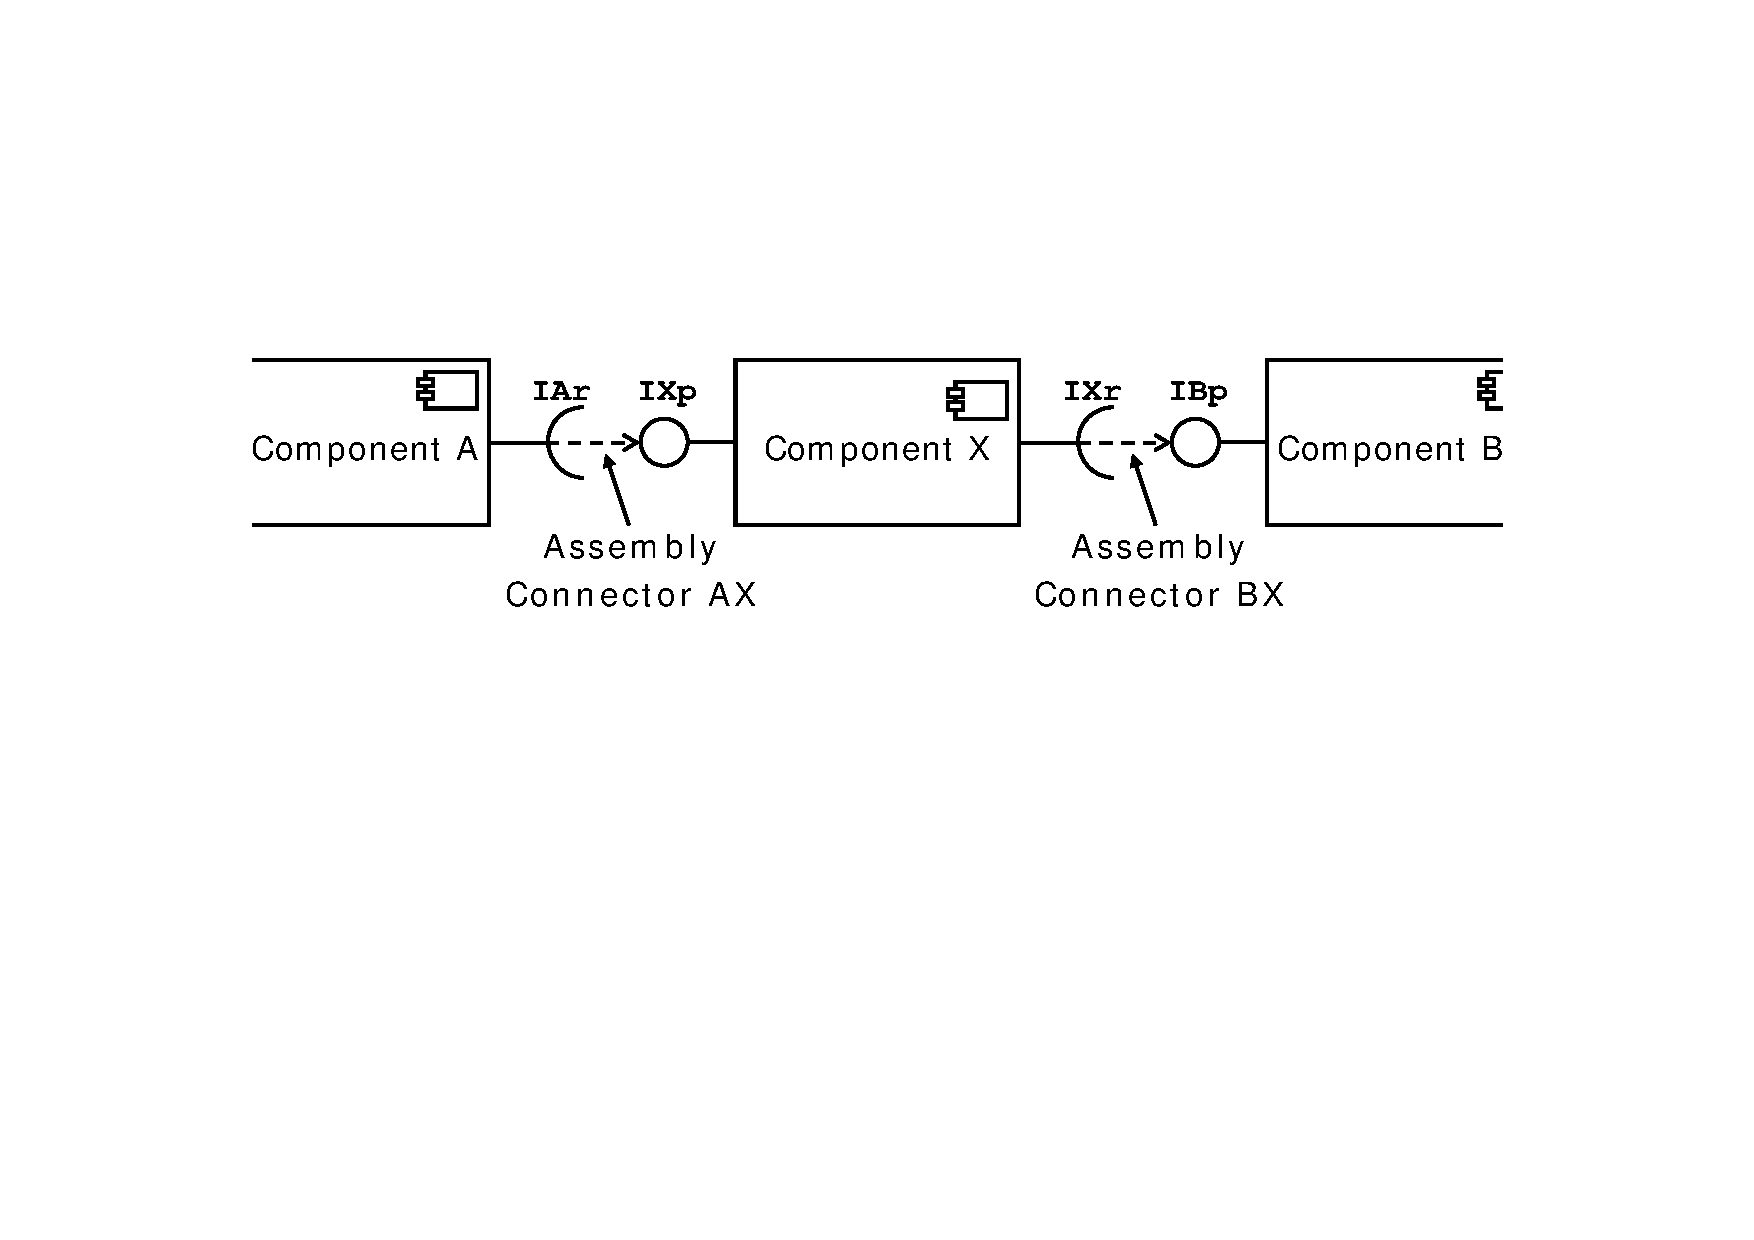
\includegraphics[width=0.80\textwidth]{./image/cm-component-substitution-01.pdf}
	\caption{Substition der Komponente X ("`Component X"') in einer bestehenden Komponentenarchitektur}
	\label{fig:cm-component-substitution-01}
\end{figure}



Abbildung \ref{fig:cm-component-substitution-01} verdeutlicht die Problematik, die sich bei der Substitution von Komponenten durch andere ergibt. Die auf der linken Seite gegebene "`Component A"' ben�tigt die Schnittstelle \texttt{IAr}. Auf der rechten Seite gibt "`Component B"' die Schnittstelle \texttt{IBp} fest vor. An dieser Stelle ist zu kl�ren, welche Komponenten (mit welchen angebotenen und ben�tigten Schnittstellen) f�r "`Component X"' verwendet werden k�nnen.

Das skizzierte Problem besteht bei der Neu"=Definition von Komponentenarchitekturen, unter Verwendung gegebener Komponenten ebenso wie bei Ersetzung bestehender (alter) Komponenten in bestehenden Komponentenarchitekturen.

Zu bedenken bleibt, dass, je nach Detailniveau respektive Typ"=Ebene der Komponenten, auf den Schnittstellen Protokolle definiert sein k�nnen und die Komponenten selbst SEFFs vorschreiben. Bei einer Komponenten-Substitution sind gegebenenfalls auch diese zu ber�cksichtigen.



\subsubsection{Co- und Contra-Varianz}
\label{sec:Co-undContra-Varianz}



\paragraph{Allgemein}



Eine g�ltige Substitution f�r eine Komponente liegt im Allgemeinen dann vor, wenn auf allen \textit{Provides Interfaces} einer Komponente
\begin{itemize}
	\item die Menge der angebotenen Dienste eine Obermenge der geforderten Dienste ist, und
	\item das angebotene Protokoll eine Sprach-Obermenge des geforderten Protokolls ist.
\end{itemize}
Umgekehrt, man spricht in diesem Fall von "`Contra-Varianz"' (siehe auch \cite{co-contra}), muss f�r alle \textit{Requires Interfaces} gelten, dass
\begin{itemize}
	\item die geforderten Dienste eine Untermenge der angebotenen Dienste sind, und
	\item das geforderte Protokoll eine Sprach-Untermenge des angebotenen Protokolls ist.
\end{itemize}

TODO:--> Signatur, wann gleich. Wird das beachtet? Einfachster Fall: nur identische Signaturen beachtet.

Gen�gen alle \textit{Provides} und alle \textit{Requires} Schnittstelle einer Komponente den oben genannten Bedingungen, kann sie (als Substitut) verwendet werden.

Um entscheiden zu k�nnen, ob Komponenten mit ihren Schnittstellen durch andere substituiert (Sub"=Typ"=Beziehung) werden k�nnen, ist es sinnvoll Protokolle, respektive Sprachen, zu verwenden, deren Inklusionsproblem entscheidbar ist. Wie bereits zuvor erw�hnt wurde, ist die Verwendung von endlichen Automaten im Komponentenmodell sehr verbreitet. Da endliche Automaten und regul�re Ausdr�cke sprach�quivalent sind, und f�r regul�re Ausdr�cke das Inklusionsproblem l�sbar ist, womit diese Problem auch f�r endliche Automaten l�sbar ist, erscheint die Entscheidung zur Verwendung von endlichen Automaten in Praxisbeispielen sinnvoll (vgl. cite{TODO}). Die andere, im Komponentenmodell-Kontext verbreitete Variante zur Darstellung von Protokollen und SEFFs, die Petri-Netze, sind kontextsensitiv, weshalb das Wortproblem ebenfalls l�sbar ist (vgl. cite{TODO}).



\paragraph{Typ-Ebenen abh�ngig}



Da Protokolle auf Schnittstellen, unabh�ngig von der Typ"=Ebene von Komponenten, definiert werden \textit{k�nnen}, gibt es keine Kopplung zwischen vorliegenden Komponenten einer bestimmten Typ"=Ebene und dem Vorkommen von Protokolle. Es ist jeweils m�glich, dass ein Protokoll definiert ist, eine Sicherheit gibt hierf�r nicht. Um dennoch die Substitutierbarkeit unter Beachtung von Protokollen pr�fen zu k�nnen, nimmt das Komponentenmodell, sofern auf einer Schnittstelle kein Protokoll definiert ist, ein Trivial"=Protokoll an. Abbildung \ref{fig:cm-trivial-protocol-01} zeigt ein Trivial-Protokoll. Bei diesem implizit angenommenen Protokoll sind Dienstaufrufe auf der Schnittstelle in beliebiger Reihenfolge m�glich.

Soll eine Komponente substituiert werden, die auf einem Teil ihrer Schnittstellen kein Protokoll definiert hat, wird f�r diese Schnittstellen das Trivial"=Protokoll (siehe Abbildung \ref{fig:cm-trivial-protocol-01}) zur Pr�fung anhand der in Kapitel \ref{sec:Co-undContra-Varianz} genannten Regeln herangezogen. Die Pr�fung ist damit problemlos wie in allen anderen F�llen m�glich.



\begin{figure}[htbp]
	\centering
		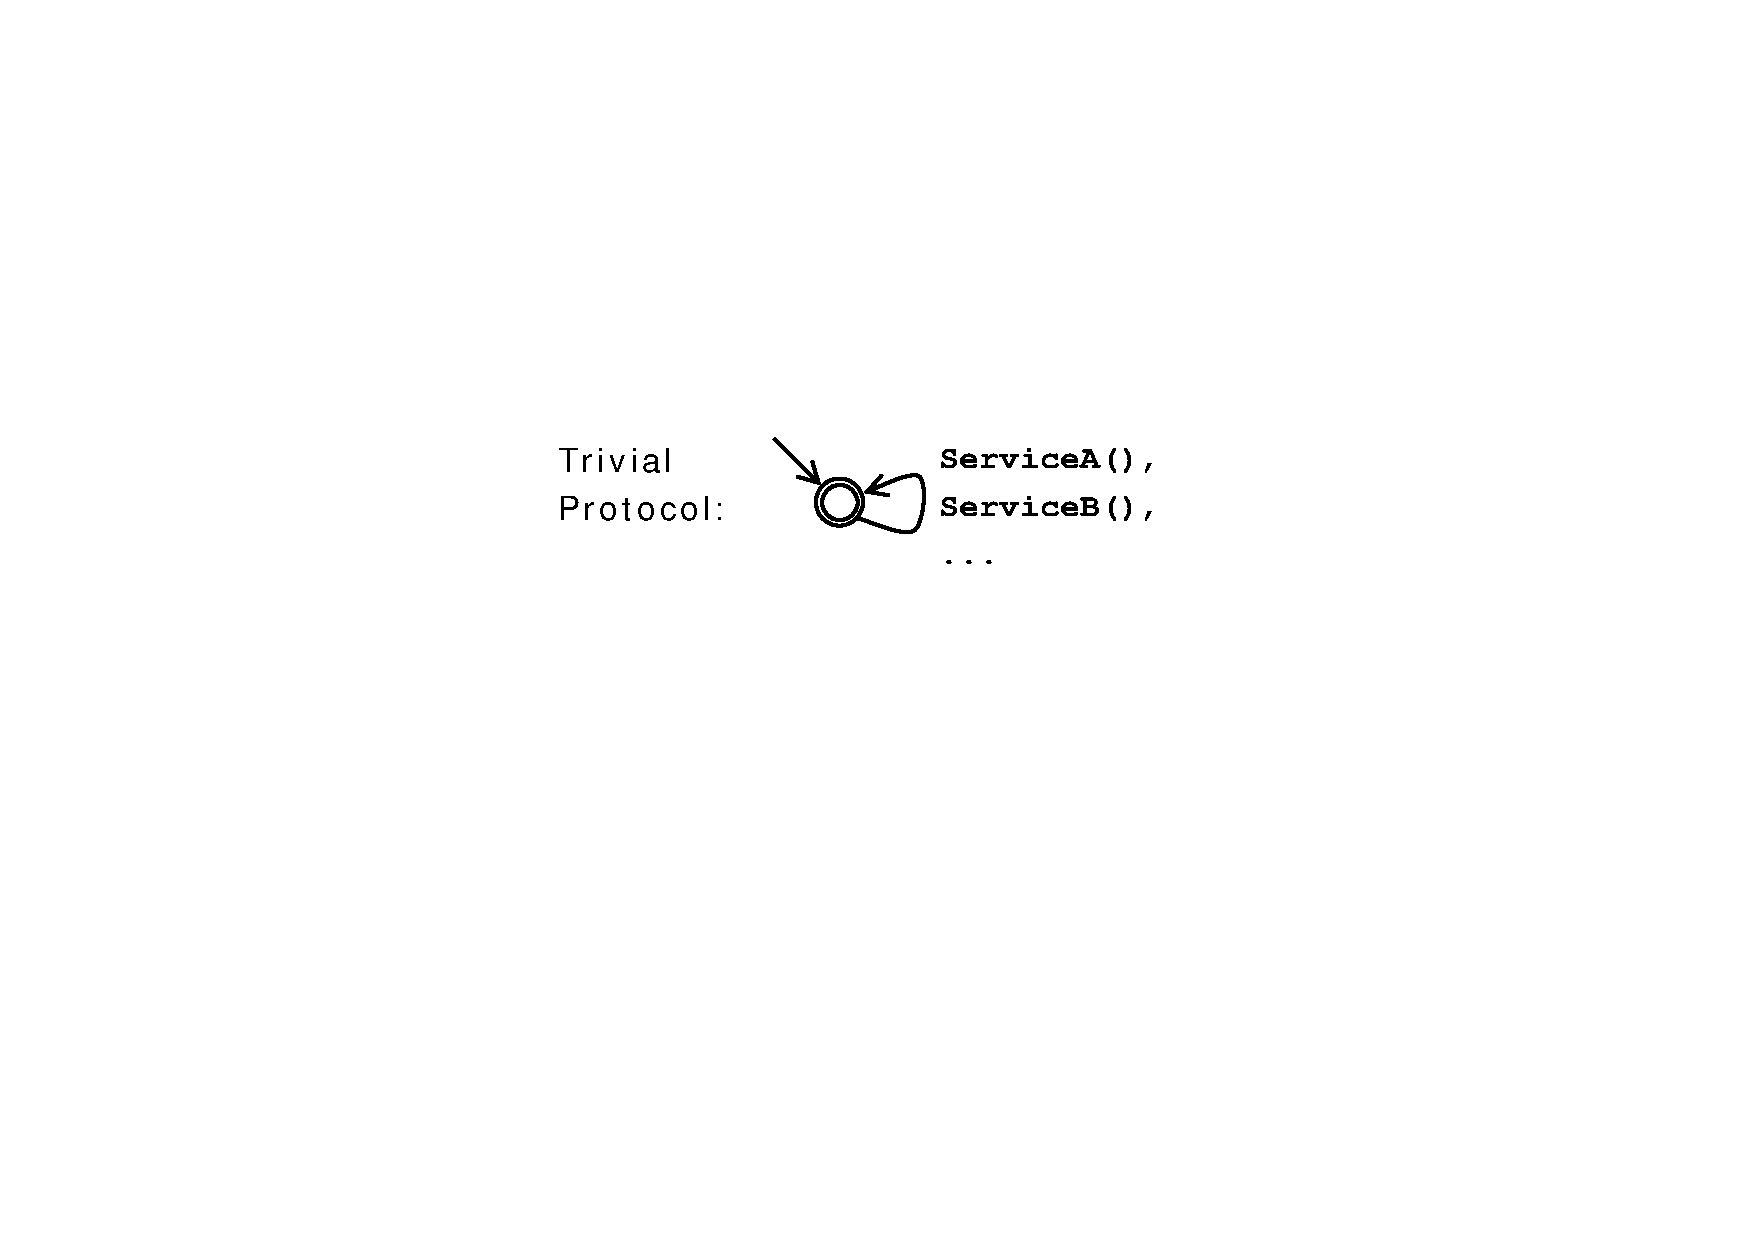
\includegraphics[width=0.45\textwidth]{./image/cm-trivial-protocol-01.pdf}
	\caption{Trivial-Protokoll; Dienstaufrufe sind in beliebiger Reihenfolge m�glich}
	\label{fig:cm-trivial-protocol-01}
\end{figure}



Der \textit{Provided Type} definiert keinerlei ben�tigte Schnittstellen. Soll ein solcher Komponenten"=Typ substituiert werden oder f�r eine Substituion verwendet werden, nimmt man auf der \textit{Requires}"=Seite implizit genau eine Schnittstelle an. Diese Schnittstelle ist leer, definiert also keine Dienste und ein Protokoll, das nur einen Endzustand besitzt, also die Leere Sprache ($L\:=\:\varnothing$) akzeptiert. Anhand der allgemein definierten Regeln wird dann �berpr�ft, ob eine Substitution g�ltig ist.

Wird eine \textit{Provided Type} oder eine \textit{Complete Type} Komponente durch eine \textit{Implementation Type} Komponente ersetzt, sollte bedacht werden, dass mit dem \textit{Implementation Type} und dem damit verbundenen SEFF das ben�tigte Protokoll berechenbar wird. Entsprechend muss das berechnete Protokoll, dass sich damit von einem vorher definierten Protokoll unterscheiden kann, f�r die Substitution valide sein.



\subsubsection{Delegations-Konnektoren}
\label{sec:Delegations-KonnektorenSubTyp}
Delegations"=Konnektoren lassen sich nicht ohne Weiteres mit den in Kapitel \ref{sec:Co-undContra-Varianz} angef�hrten Regeln auf Validit�t pr�fen, da sie zun�chst gleichartige Schnittstellentypen miteinander verbinden. Betrachtet man bei \textit{Provides}"=Delegations"=Konnektoren die �u�ere Schnittstelle als \textit{Requires}"=Schnittstelle und bei \textit{Requires}"=Delegations"=Konnektoren die �u�ere Schnittstelle als \textit{Provides}"=Schnittstelle, k�nnen die bereits bekannten Regeln aus Kapitel \ref{sec:Co-undContra-Varianz} verwendet werden.

Auf der \textit{Provides}"=Seite darf die �u�ere Schnittstelle also nur die gleiche Schnittstelle wie die innere anbieten oder diese eingeschr�nkt anbieten. Dies f�hrt dazu, dass alle Dienstaufrufe auf definierte innere Schnittstellen geleitet werden. Auf der \textit{Requires}"=Seite darf die �u�ere Schnittstelle gleich viel wie die innere Schnittstelle oder mehr verlangen. Auf diese Weise k�nnen zwar nicht ben�tigte Anforderungen definiert werden, anders herum laufen jedoch keine Dienstanfragen ins Leere.



\subsubsection{Einschr�nkungen}
\label{sec:EinschraenkungenSubTyp}
Ob die in diesem Kapitel genannten Regeln f�r die Substitution von Typen eingehalten werden, h�ngt von der konkreten Implementierung des Komponenten"=Meta"=Modells ab. Zun�chst einmal gibt das Komponenten"=Meta"=Modell, das beschrieben wurde, lediglich einen Satz von allgemeinen Regeln vor, kann die Einhaltung jedoch nicht aktiv �bernehmen. Implementierungen des Komponenten"=Meta"=Modells sind jedoch daran gehalten, solche �berpr�fungen, die nicht zuletzt auch konsistenz"=erhaltend sind, zu definieren.

Es sollte bedacht werden, dass weder f�r Protokolle noch SEFFs vom Komponenten("=Meta"=)modell spezielle Typen vorgegeben werden. Entsprechend m�ssen die zu definierenden Pr�fungs"=Algorithmen austauschbar sein. Eine Implementierung des Komponentenmodells sollte daher im Kern keine festen Typen vorsehen, sondern eine Erweiterbarkeit um "`Pr�fmodule"' �ber \textit{Plugin}"=�hnliche Mechanismen, die dann auf einem konkreten Typ funktionieren.

Allgemeine Bemerkungen zur Validierung des Komponentenmodells finden sich in Kapitel \ref{sec:ValidierungvonModellinstanzen}.



\subsection{Allokation}
\label{sec:Allokation}



\begin{figure}[htbp]
	\centering
		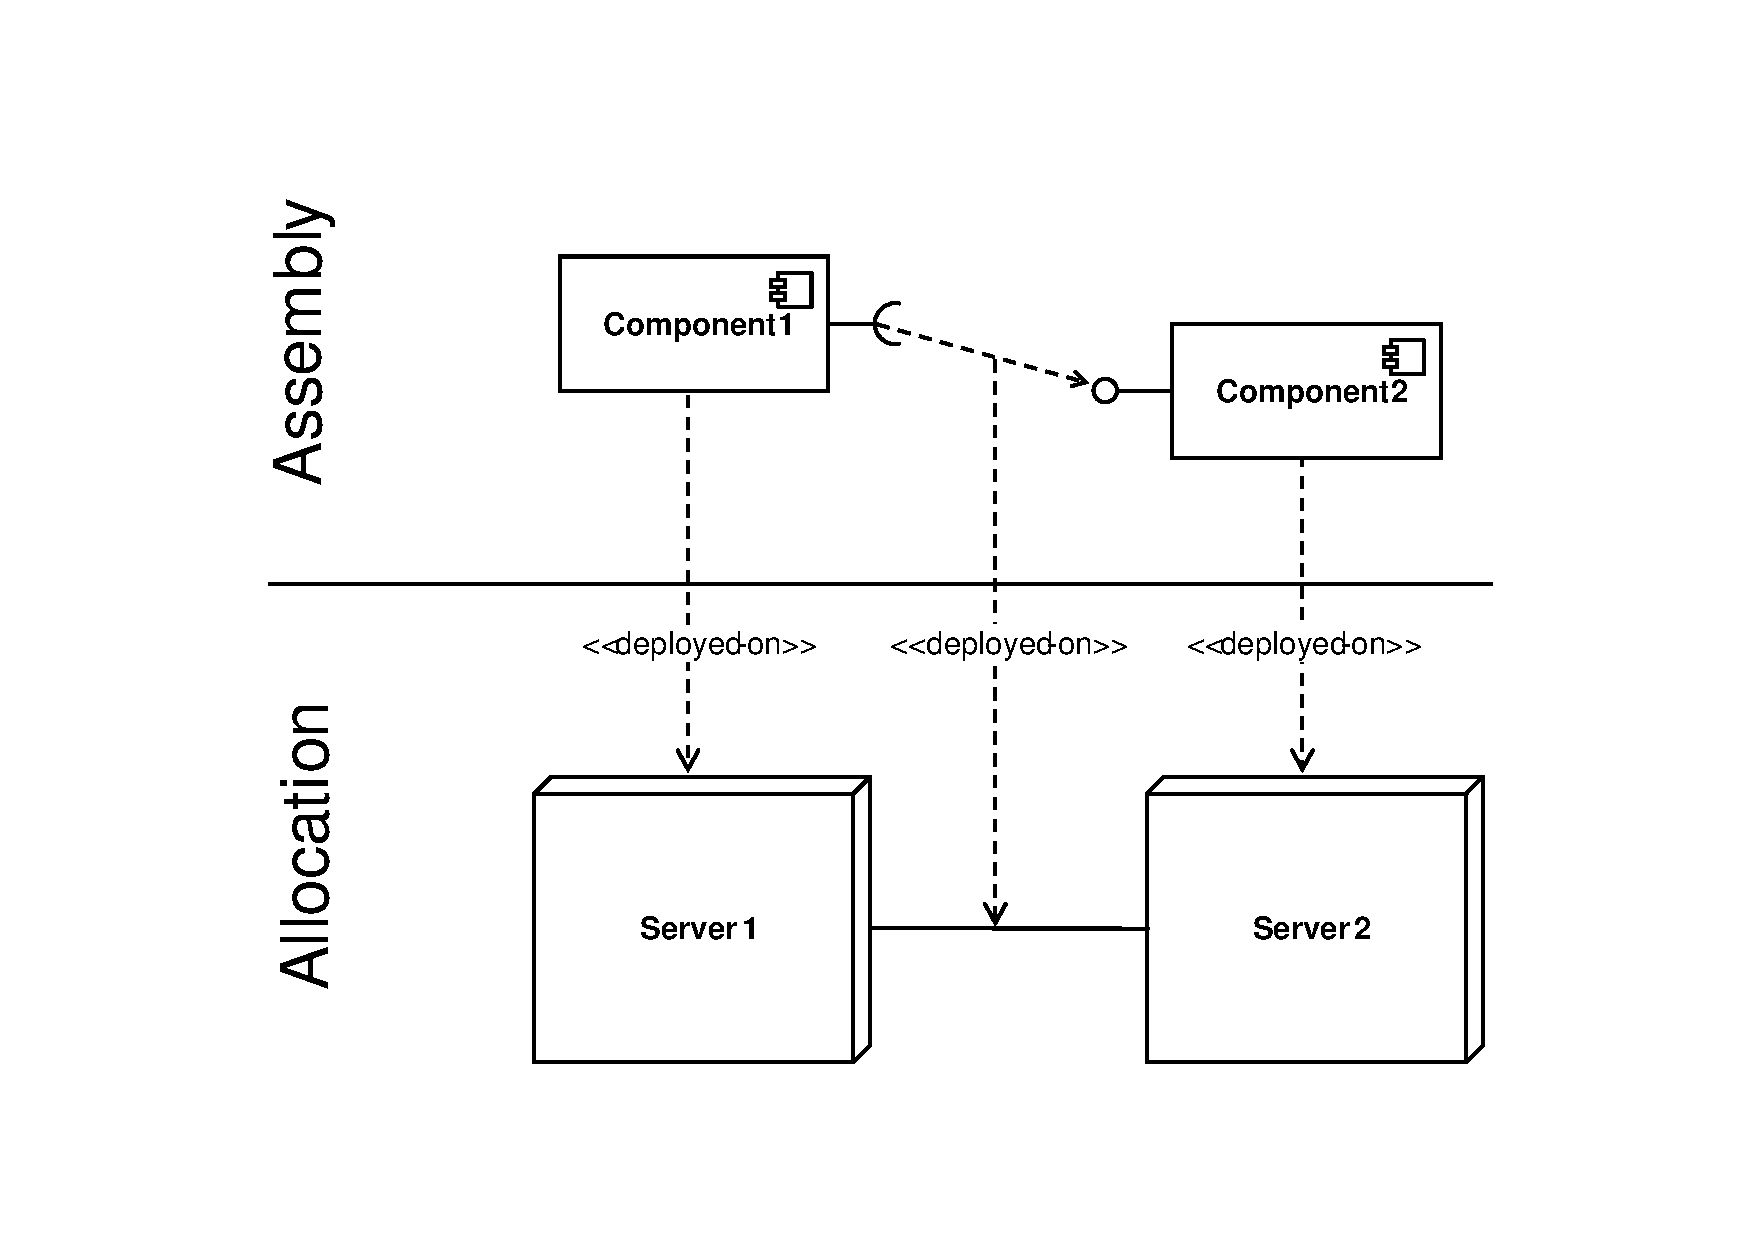
\includegraphics[width=0.60\textwidth]{./image/cm-assembly-allocation-01.pdf}
	\caption{Assembly und Allokation (nach \cite{PalladioCMNeuSlides}, S. 26)}
	\label{fig:cm-assembly-allocation-01}
\end{figure}



In Abbildung \ref{fig:cm-assembly-allocation-01} wird versucht die Begrifflichkeiten der Assembly und der Allokation (\textit{Allocation}) zu unterscheiden, so wie sie im Kontext des Palladio Komponentenmodells verwendet werden. Diese Sprachregelungen m�ssen sich nicht zwangsl�ufig mit anderen Definitionen decken. 

TODO:

was ist deployment?


System construction
Assembly of components
Deployment (Installation)
Allocation of components on resources 
Both can be done independently
Both define the context of a component



\subsection{Assembly}
\label{sec:Assembly}



\subsubsection{Differenzierung von Assemblies gegen�ber Composite Components}
\label{sec:DifferenzierungvonAssemblieszuCompositeComponents}



In der Sprachwelt des Komponentenmodells sind \textit{Assemblies} und \textit{Composite Components} strikt zu unterscheiden (vgl. \cite{PalladioCMNeuSlides}, S. 27f).



\paragraph{Composite Component}
Wie bereits beschrieben, setzt sich eine \textit{Composite Component} aus anderen Komponenten zusammen. Zum Zeitpunkt des \textit{Deployments} ist das Innere, die Realisierung einer \textit{Composite Components} unsichtbar. Daher ist es einem \textit{System Deployer} nicht m�glich, eine \textit{Composite Component} �ber verschiedene Ausf�hrungsungsumgebungen (\textit{Execution Environment}) zu verteilen.



\paragraph{Assembly}
Auch \textit{Assemblies} (im Komponentenmodell auch \textit{Component Assemblies} genannt) werden aus Komponenten aufgebaut. Im Gegensatz zur \textit{Composite Component} ist das Innere einer \textit{Assembly} jedoch zum Zeitpunkt des \textit{Deployments} f�r den \textit{System Deployer} sichtbar. Dies erm�glicht, dass innere Komponenten einer Assembly auf unterschiedlichen Ausf�hrungsumgebung allokiert werden k�nnen.
Das bedeutet, dass einzelne Komponenten (ohne Kopien) durch ihre Erfassung in einer Assembly zur gleichen Zeit nicht auf unterschiedlichen Ausf�hrungsumgebungen ausgef�hrt werden k�nnen. Sehr wohl kann jedoch komponentenweise verteilt werden. 



\begin{figure}[htbp]
	\centering
		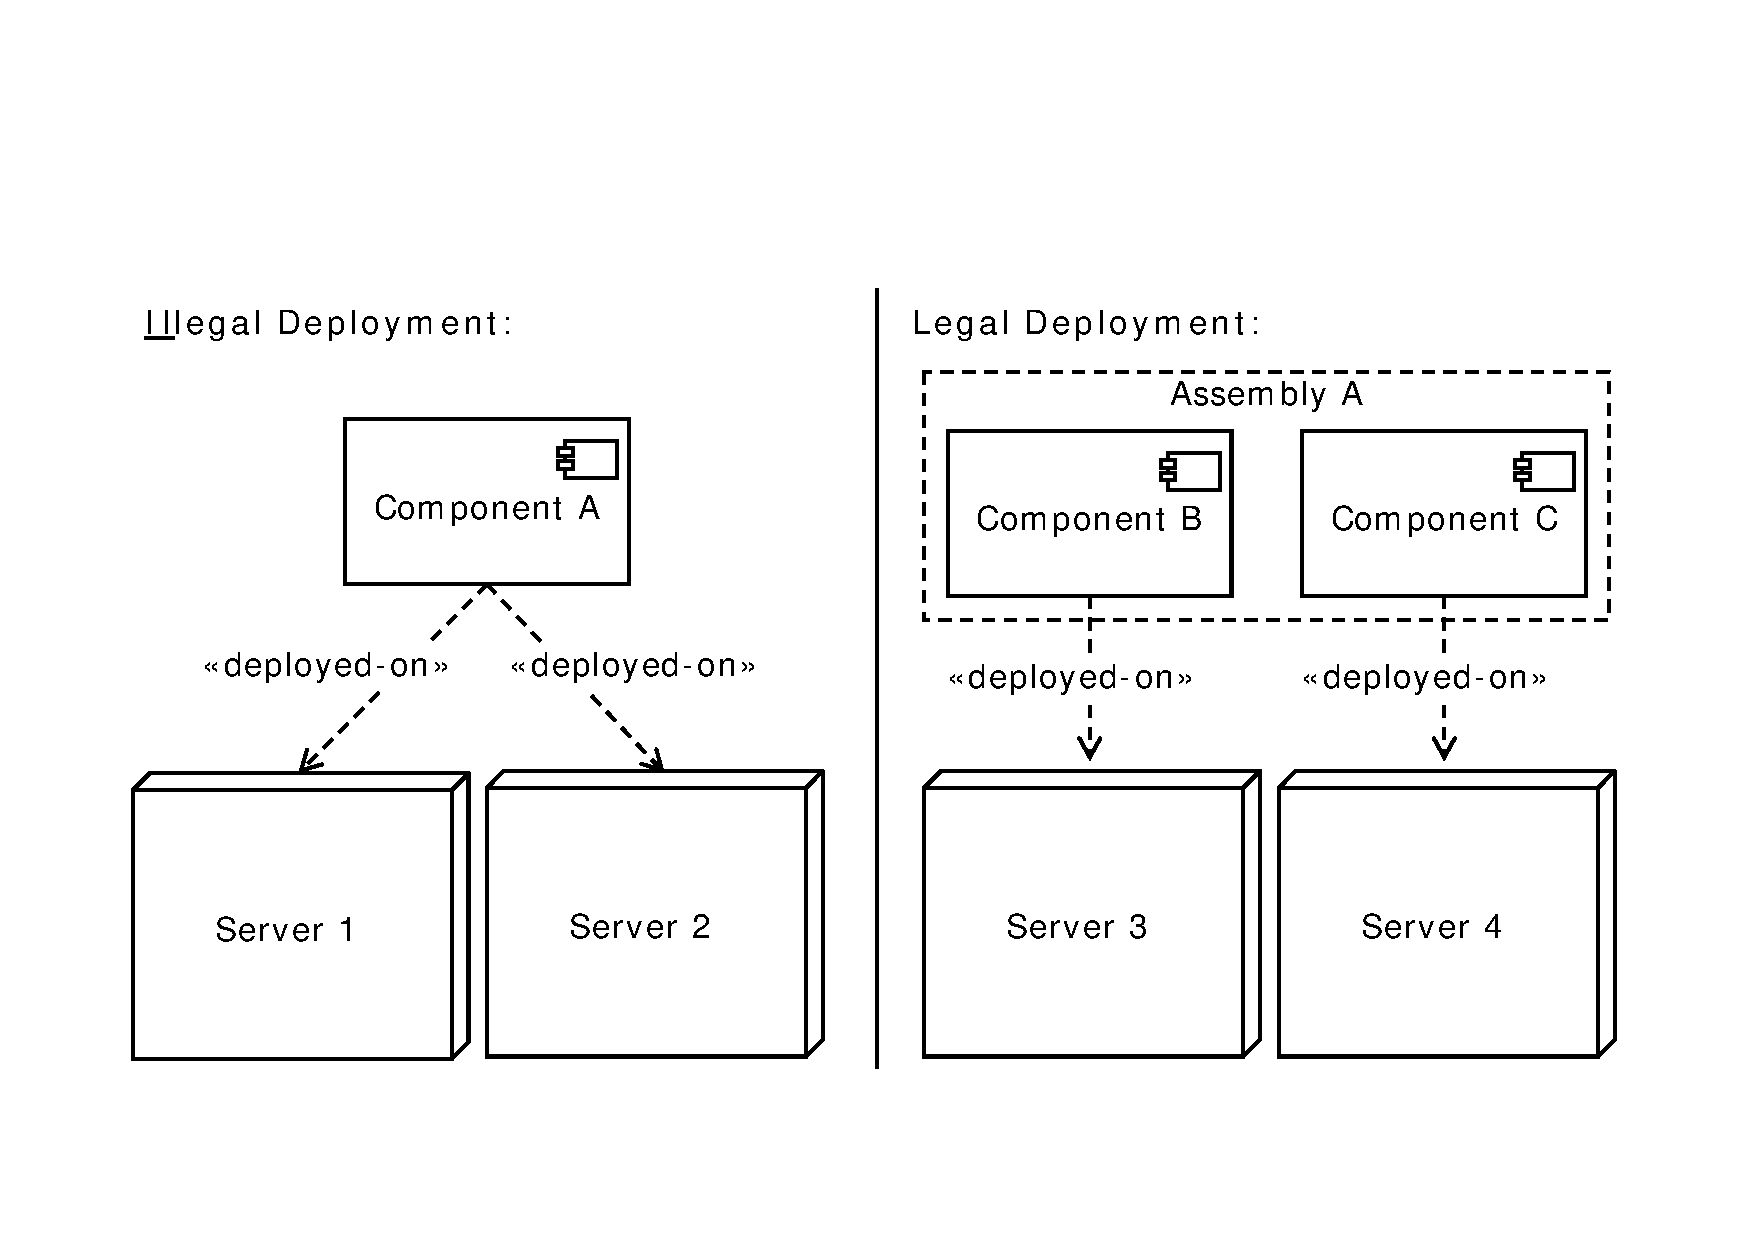
\includegraphics[width=0.80\textwidth]{./image/cm-il-legal-deployment-01.pdf}
	\caption{Illegales und legales \textit{Deployment} von Komponenten}
	\label{fig:cm-il-legal-deployment-01}
\end{figure}



In Abbildung \ref{fig:cm-il-legal-deployment-01} wird gegen�ber gestellt, welche \textit{Deployment}formen legal sind. Auf der linken Seite wird eine ung�ltige Variante dargestellt, bei der eine Komponente ("`Component A"') auf verschiedene Ressourcen ("`Server 1 und Server 2"') verteilt werden soll. Auf der rechten Seite erfolgt ein g�ltiges \textit{Deployment}. Die Komponenten "`Component B"' und "`Component C"' liegen in einer \textit{Assembly}. Zugleich werden sie jeweils auf eigene Ressourcen verteilt. Eine ebenfalls g�ltige Variante w�re die Verteilung der Komponenten B und C auf die gleiche Ressource.

Therefore, it is possible that its inner components can be allocated on different execution environments. An assembly itself cannot be composed (as it is no component) but it can be extended (with other components or assemblies) or it can be transformed into a (composite) component by making its internal structure invisible for the system deployer. 




\subsubsection{Assemblydefinition}
\label{sec:..}






\subsection{Kontext}
\label{sec:Kontext}



\subsection{Identit�t}
\label{sec:Identitaet}
Komp. mit gleichen prov und req interf. kann != anderer sein, die die gleichen schnittstellen bietet! --> ID.

Was hat ID, wie ich equals und == definiert?

Typisierte IDs --> M�glichkeiten mit EMF bedenken

In Relationen werden �blicherweise IDs verwendet



\subsection{Anotationen}
\label{sec:Anotationen}



\subsection{Weitere F�higkeiten}
\label{sec:WeitereFaehigkeiten}
Parametrisierte Vertr�ge, QoS, ...



\subsection{Validierung von Modellinstanzen}
\label{sec:ValidierungvonModellinstanzen}
TODO: Erweiterungen zu Kapitel \ref{sec:Typ-Spezialisierung}. Insbesondere auf QoS-Attributen, parametrisieren Vertr�gen und SEFFs (pr�fen ob eine substitution zul�ssig: erhaltung der seff-eigenschaften denkbar).
TODO: Unterscheidung: Validierung vs. Konsistenz.



\subsection{Einschr�nkungen}
\label{sec:EinschraenkungenCM}



\subsection{Ausblick auf die Entwicklung}
\label{sec:AusblickaufdieEntwicklung}
TODO: Ein neues Paper, das das aktuelle Komponentenmodell beschreibt, wird in K�rze unter \cite{PalladioCMNeu} ver�ffentlicht.




------------------------------------


\textbf{TODO:}
- Parametrisierte Vertr�ge: Auswirkungen auf Requires-Schnittstelle: nicht mehr alles notwendig
- Komponente ruft sich selbst auf: wann unendliche rekursion, wann auf welcher ebene erlaubt --> insbesondere unbekannt in CCs
- mehrere konnektoren auf eine provided schnittstelle: zustand nicht mehr unterscheidbar.: In der Umkehrung kann eine angebotene Schnittstelle jedoch �ber \texttt{0..*} ben�tigte Rollen verwendet werden. Damit bleibt die graphische Notation nicht eindeutig...
- keine Unterst�tzung f�r Zust�nde �ber mehrere schnittstellen hinweg.
- Typ-Ersetzbarkeit: Verschiedene Betrachtungsm�glichkeiten / Interoperabilit�tsniveaus: Signatur, Protokoll, QoS --> Grafik
Um entscheiden zu k�nnen, ob Komponenten mit ihren Schnittstellen durch andere substituiert (Sub"=Typ"=Beziehung) werden k�nnen, ist es sinnvoll Protokolle, respektive Sprachen, zu verwenden, deren Inklusionsproblem entscheidbar ist.
- Anotationen wann und wo?
- QoS-F�higkeiten


------------------------------------





Neu wird im Palladio Komponentenmodell der Begriff des "`Kontexts"' eingef�hrt. Dabei wird unterschieden in
\begin{itemize}
	\item "`Verdrahtung"' von Komponenten untereinander im Sinne einer Komponentenarchitektur (\textit{System Construction / Assembly Composition}) und
	\item Allokation von Komponenten auf Ressourcen (\textit{Deployment / Allocation}).
\end{itemize}
Das Ziel des dahinter liegenden Konzepts ist eine M�glichkeit zur Unterscheidung von Komponenteneigenschaften je nach ihrem konkreten Verwendungskontext. So kann die \textit{gleiche} Komponente, unterschieden nach dem Typ auf einer der oben genannten Ebenen, ein unterschiedliches Verhalten je nach Kontext aufweisen.

Nach der \textit{Assembly Composition} richten sich die aufgerufenen und aufrufenden Dienste. Damit k�nnen z. B. die Aufrufparameter von Diensten variieren. Es �ndern sich also prim�r funktionale Eigenschaften einer Komponente. Mit der \textit{Allocation} variiert unter anderem die Ausf�hrungsumgebung. Dies hat z. B. Auswirkungen auf die Ausf�hrungsgeschwindigkeit, Sicherheit oder die Konfiguration zur Ausf�hrung einer Komponente. Vornehmlich sind hiervon also nicht"=funktionale Eigenschaften betroffen.

Zus�tzlich zu den beschriebenen statischen Strukturen bietet das Komponentenmodell Unterst�tzung f�r beliebige Zusatzattribute, die f�r Entit�ten (Schnittstellen und Komponenten, Protokolle u. a.) vergegeben werden k�nnen. Hierunter fallen ebenfalls QoS (\textit{Quality of Service}) Attribute, f�r die das Komponentenmodell eine Berechnungsgrundlage bietet. Das Komponentenmodells erm�glicht mit seinen Daten die Auswertung von parametrisierten Vertr�gen, wie sie von Reussner in \cite{reussner01i} beschrieben werden.




---------------------------------


\newpage
\section{ALT}



\subsection{Fragestellungen}
\label{sec:Fragestellungen}
Der Diplomarbeit liegen unter anderem die folgenden Fragestellungen zu Grunde:
\begin{itemize}
	\item Widersprechen sich Modellierungskonzepte des Palladio Komponentenmodells? Sind Einschr�nkungen des Komponentenmodells erkennbar? Wurden auf Grund fehlender formaler Manifestierung des Modells Unvollst�ndigkeiten �bersehen? Welche Semantik verbirgt sich hinter spezifischen Modellierungskonstrukten?
	\item Das Palladio Komponentenmodell ist zu kleinen Teilen nur implizit in den K�pfen der Mitglieder der Palladio-Gruppe vorhanden. Gibt es Widerspr�che in den impliziten Annahmen?
	\item Welche der konzeptionellen Aspekte des Palladio Komponentenmodells lassen sich mit den gew�hlten Hilfsmitteln wie UML, ECORE, EMF und anotiertem Java abbilden?
	\item Welche Aspekte lassen sich nicht abbilden und aus welchen Gr�nden scheitert diese Abbildung. Welche Einschr�nkungen gelten f�r UML, ECORE, EMF und anotiertem Java? Welche Erweiterungen der (Abbildungs-) Modelle m�ssten vorgenommen werden.
	\item Welche Wege bieten sich zur Modellierung an? Welche Alternativen gibt es bei der Modellierung? Aus welchen Gr�nden wurden welche Alternativen gew�hlt? Gibt es gleichwertige Alternativen oder widerspr�chliche Herangehensweisen?
	\item Wie lassen sich variable Zusatzattribute im Meta-Modell unterbringen und wie finden sich diese Zusatzattribute im generierten Modell-Code bzw. einem Modell-Editor wieder?
	\item Welche technologischen und konzeptionellen Einschr�nkungen bringen die verwendeten Generatoren und Transformatoren mit sich?
\end{itemize}



\subsection{Annahmen}
\label{sec:Annahmen}


\begin{itemize}
	\item UML, ECORE, EMF und anotiertes Java m�ssen m�chtig genug sein, um darin alle Konzepte des Palladio Komponentenmodells abzubilden.
	\item Um die bereits angesprochenen variablen Zusatzattribute zu Modell-Entit�ten zu erm�glichen, ist es notwendig, dass dies durch die Meta-Modellierung auf den folgenden Ebenen unterst�tzt wird: UML, ECORE, EMF und anotiertem Java. F�r UML bedeutet dies, dass das Meta-Modell f�r ein gegebenes Zusatzattribut dynamisch vom Kern-Meta-Modell (Meta-Modell ohne Zusatzattribute) referenziert werden kann.
	\item Ferner wird angenommen, dass der zu verwendende Generator von EMF ausreichend m�chtig ist, um alle Aspekte des Palladio Komponentenmodells in anotiertem Java abzubilden.
	\item Die M�glichkeiten die Transformationen von GMF eigenen Bed�rfnissen anzupassen m�ssen ausreichend gro� sein, um einen den Benutzerbed�rfnissen entsprechenden Editor generieren zu k�nnen.
	\item Wie bereits angesprochen, muss davon ausgegangen werden, dass der in Kapitel ref{TODO:sec:Gesamtprozess} skizzierte Prozess in mehreren Iterationen (insbesondere auf Grund der "`konzeptionellen Variabilit�t"' des Palladio Komponentenmodells) durchlaufen werden muss. Da nicht davon ausgegangen werden kann, dass jegliche generierten Modelle und Code ohne manuelle Nachpflege verwendet werden k�nnen, ergibt sich zwingend die Anforderung, dass der EMF-Generator und auch GMF funktionierende "`Merge"'-Mechanismen implementieren, die verschiedene Modellversionen (zumindest nach kleineren �nderungen) unter Erhaltung manueller �nderungen zusammenf�hren k�nnen. Nur mit einem solchen Mechanismus l�sst sich der iterative Prozess sinnvoll durchf�hren.
	
	Zum Zeitpunkt der Niederschrift dieses Proposals wird ein solcher Merge"=Mechanismus von Merlin nicht unterst�tzt.
\end{itemize}

Sind nicht alle hier dargestellten Annahmen erf�llt, hat dies direkte Auswirkungen auf die Umsetzung der Diplomarbeit. Daher sind die hier genannten Annahmen auch im Zusammenhang mit den Risiken zur Umsetzung der Diplomarbeit (siehe Kapitel \ref{sec:Risikomanagement}) zu sehen.



\subsection{Fehlerquellen}
\label{sec:Fehlerquellen}
TODO



\subsection{Einschr�nkungen}
\label{sec:Einschraenkungen}
Im Rahmen der Diplomarbeit ist \textit{nicht} geplant, einen vollst�ndigen, industriellen Standards gen�genden, GUI-Editor f�r das Palladio Komponentenmodell zu erzeugen. Im Vordergrund steht die Modellierung der EMF-Darstellung des dem Editor als Basis dienenden Komponenten-Meta-Modells und die Erprobung m�glicher Wege zur Generierung eines vollst�ndigen Editors.



\subsection{Risikomanagement}
\label{sec:Risikomanagement}
Die Durchf�hrung der Diplomarbeit unterliegt vielf�ltigen Risiken. �ndern sich Grundannahmen, wie in Kapitel \ref{sec:Annahmen} dargestellt, kann ein erfolgreicher Abschluss der Diplomarbeit gef�hrdet sein. Um Risiken zu minimieren werden an dieser Stelle f�r wahrscheinliche Risiken Auswege aufgezeigt.

\paragraph{Konzeptioneller Wandel im Palladio Komponentenmodell} Wie bereits mehrfach in vorangegangenen Kapiteln erw�hnt wurde, ist das Palladio Komponentenmodell aktiver Gegenstand von Forschungsarbeit. Damit verbunden ist das Risiko, dass sich Modell"=Konzepte �ndern k�nnen, Modell"=Erweiterungen erg�nzt werden und nicht mehr ben�tigte oder problematische Teile des Modells wegfallen k�nnen. Um das Risiko in diesem Bereich einzugrenzen, bieten sich zwei Strategien an:
\begin{enumerate}
	\item Wird die Version des Komponentenmodells f�r die Diplomarbeit eingefroren, kommen konzeptionelle �nderungen in der Diplomarbeit nicht zum Tragen. Dieser Ansatz birgt jedoch die Gefahr, dass die Modellversionen in der Diplomarbeit und der realen Entwicklung stark divergieren.
	\item �nderungen am Komponentenmodell k�nnen genau beobachtet werden und nur wenn �nderungen als unkritisch eingestuft werden, flie�en sie in die Diplomarbeit ein. Dies hat den Vorteil, dass das Meta-Modell aus der Diplomarbeit st�rker dem realen Stand entspricht.
\end{enumerate} 

\paragraph{Annahmen nicht erf�llt} Sind Annahmen, die in Kapitel \ref{sec:Annahmen} festgestellt wurden, nicht erf�llt, sind hiermit die gr��ten Projektrisiken verbunden. Je nachdem, zu welchem Zeitpunkt im Prozess die nicht erf�llten Annahmen zum Tragen kommen, ist anzunehmen, dass die Erf�llung aller sp�teren Teile des Prozesses nur noch unwahrscheinlich ist. Das bedeutet, dass Abstriche im Umfang der Diplomarbeit zu erwarten sind. Um diesen Ausfall abzumildern, k�nnten beispielsweise f�r die verwendeten Modelle und Werkzeuge Alternativ-Produkte verwendet werden.

\paragraph{Verf�gbarkeit verwendeter Werkzeuge} Sollten im Rahmen der Diplomarbeit verwendete Werkzeuge nicht mehr verf�gbar sein (etwa aus Gr�nden von Lizenzproblemen), sollte versucht werden, geeignete Alternativen zu finden und zu verwenden. Insbesondere im Falle von GMF baut die Diplomarbeit darauf, dass dieses Werkzeug, wie in der Vergangenheit, weiterentwickelt wird. Da hinter GMF ma�geblich IBM und Borland mit professionellen, bezahlten Entwicklern stehen, ist es notwendig, dass diese Firmen weiterhin Interesse an der Entwicklung haben und keinen strategischen Wechsel vollziehen. Zudem ist die Diplomarbeit davon abh�ngig, dass das Projekt ausreichend schnell voranschreitet und in einen stabilen Zustand gelangt.

Sollten Probleme mit GMF auftreten, bietet sich ein R�ckgriff auf Merlin oder die bis dahin letzte stabile Entwicklerversion an.

\paragraph{Vertikaler Prototyp}
Zur weiteren prophylaktischen Minimierung von Risiken wurde bereits erfolgreich (wenn auch mit gewissen Einschr�nkungen) ein vertikaler Prototyp unter Verwendung von Merlin erzeugt. Als einer der ersten Schritte der Diplomarbeit ist ein weiterer vertikaler Prototyp geplant, der sp�ter auch Basis darauf folgender Iterationen sein wird. Dieser soll GMF verwenden und variable Zusatzattribute testen.




\subsection{Zeitplanung}
\label{sec:Zeitplanung}
Zeitplanung in der Retrospektive







%____________________________________________________________________________________________________________
%____________________________________________________________________________________________________________
%____________________________________________________________________________________________________________
%
% "`Hineinlinken"' von Zusatzinformationen in UML muss m�glich sein. Zun�chst Linking und Referenzieren ausprobieren.
%
% Wichtig: Trennung von Shapes und Entit�ten
%
% KM3 Eclipse --> Ascii-Repr�sentation


	
	
	% Anhang
	\appendix
	% $Log$
% Revision 1.2  2006/02/11 14:35:02  kelsaka
% - cc im hinblick auf kontext �berarbeitet
%
% Revision 1.1  2006/02/11 13:00:05  kelsaka
% - anhang ausgegliedert
%


	

\chapter{Anhang}
\label{sec:Anhang}



\section{UML}



% Abbildungsverzeichnis
\addcontentsline{toc}{section}{Abbildungsverzeichnis} %\protect\numberline{1}{Abbildungsverzeichnis}}
\lhead{Abbildungsverzeichnis} \chead{} \rhead{\thepage}
\listoffigures



%Literaturverzeichnis
\newpage
\addcontentsline{toc}{section}{Literaturverzeichnis}
\lhead{Literaturverzeichnis} \chead{} \rhead{}
% \cite* % Verursacht [] vor dem Literaturverzeichnis; ausserdem nur noch Anzeige verwendeter Literatur.
\bibliographystyle{ieeetrans}
\bibliography{Literaturverzeichnis}



\section{Selbstst�ndigkeitserkl�rung}
\label{sec:Selbststaendigkeitserklaerung}
Ich erkl�re hiermit, dass ich diese Diplomarbeit selbstst�ndig angefertigt habe und alle Teile, die w�rtlich oder inhaltlich anderen Quellen entstammen, als solche kenntlich gemacht und in das Literaturverzeichnis aufgenommen habe. Diese Arbeit wurde weder in dieser noch einer �hnlichen Form einer anderen Pr�fungsbeh�rde vorgelegt.

\ \\

Harkebr�gge, den \today{}

 \ \\ \ \\

------------------------------

\scriptsize{Klaus Krogmann}
\normalsize




	
	
	
	% Abbildungsverzeichnis
	\addcontentsline{toc}{section}{Abbildungsverzeichnis}
	\lhead{Abbildungsverzeichnis} \chead{} \rhead{\thepage}
	\listoffigures
	

	%Literaturverzeichnis
	\newpage
	\addcontentsline{toc}{section}{Literaturverzeichnis}
	\lhead{Literaturverzeichnis} \chead{} \rhead{}
	% \cite* % Verursacht [] vor dem Literaturverzeichnis; ausserdem nur noch Anzeige verwendeter Literatur.
	\bibliographystyle{ieeetrans}
  \bibliography{Literaturverzeichnis}
  	
	% Glossar
	%\newpage
	%\lhead{Glossar} \chead{} \rhead{\thepage}
	%\addcontentsline{toc}{section}{Glossar}
	%\printglossary
	%% $Log$
% Revision 1.1  2006/01/05 16:46:14  kelsaka
% - initial creation
%
% Revision 1.1  2006/01/03 10:37:55  kelsaka
% - move to folder proposal
%
% Revision 1.1  2005/12/30 15:16:18  kelsaka
% initial creation
%
%


\abbrev{Tag}{Kennzeichnungssymbol TODO}

% Kann unsortiert bleiben!!!
%\abbrev{Administrator}{Verwalter eines Softwaresystems oder eines Softwareprogrammes.}
%\abbrev{Algorithmus}{Eine zur L�sung eines bestimmten Problems oder einer bestimmten Problemklasse m�gliche Vor\-ge\-hens\-wei\-se/-folge.}
\abbrev{Analyse}{Analysen werden in Ride.NET von Analyseplugins durchgef�hrt. Analysen ermitteln Zusatzinformationen zu einem gegebenen Modell wie beispielsweise Performance-Vorhersagen oder Kontrollfluss-Visualisierungen.}
\abbrev{Anforderungen}{Anspr�che, denen das zu entwickelnde Softwaresystem entsprechen muss. Die A. an
ein Softwaresystem werden in der Anforderungsdefinition festgehalten.}
\abbrev{Anforderungsdefinition}{Bei oder vor der Softwareentwicklung entstehendes Dokument, in dem
funktionale, nichtfunktionale und generelle Anforderungen an die zu entwickelnde Software festgehalten werden.
Die A. stellt oftmals die Vertragsgrundlage bei Entwicklungsauftr�gen von Softwaresystemen dar.}
\abbrev{Antwortzeit}{Im Zusammenhang mit der Benutzerschnittstelle stellt die Antwortzeit eine nichtfunktionale Anforderung dar, die angibt, nach welcher Zeit ein Benutzer die Antwort auf seine Eingaben vom System erh�lt. F�r umfangreichere Berechnungen w�re dies die Zeit, nach der die Berechnungen abgeschlossen sind und dem Benutzer angezeigt werden k�nnen. Siehe auch \textit{Reaktionszeit}.}
\abbrev{Anwendungsfall}{Beschreibung eines speziellen Benutzungsszenarios der zu entwickelnden Software.}
\abbrev{Anwendungsfalldiagramm}{Diagrammform in der UML, in der Anwendungsf�lle der zu entwickelnden Software dargestellt sind.}
\abbrev{Artefakte}{(auch Softwareartefakte) Umfasst die Dokumentation, den Quellcode und sonstige softwarebeschreibende Informationen. Zumeist ist die elektronische Form dieser Daten gemeint. Ausgedehnt auf ein Projekt umfassen die Artefakte alle Projektinformationen (siehe auch Projekt).}
%\abbrev{Benutzer}{auch Nutzer oder User; der (End-)Benutzer eines Softwaresystemes.}
\abbrev{Bibliotheken}{Sammlung von Programmen/Funktionen, die gebrauchsfertig bei Programmierung eines
Programms zur Verf�gung stehen (k�nnen), wenn sie im Lieferumfang eines Compilers enthalten sind. B. werden je
nach Bedarf durch einen Aufruf in
Programmsegmente eingebunden.}
%\abbrev{Browser}{z. B. Navigator von Netscape, Internet Explorer von Microsoft, Mosaic...  Zeigt die von einem Server bereitgestellten Dokumente (meist in HTML) an. Er dient auch als Plattform, um Applets auszuf�hren.}
\abbrev{Bug}{Fehler oder Absturz verursachender Quelltext in
einem Software-System.}
\abbrev{C\#}{Ausgesprochen: "`C Sharp"'. Moderne objektorientierte Programmiersprache aus der Feder von Microsoft mit starken Anlehnungen an Java und C++.}
\abbrev{C0-Test}{Bei diesem Test m�ssen alle Anweisungen eines Programms mindestens einmal durchlaufen werden (Anweisungs�berdeckung). Ziel des C0-Tests ist das Finden von Programmteilen, die nicht ausf�hrbar sind. Bei dem Test handelt es sich um ein notwendiges aber nicht hinreichendes Testkriterium. Vorzugsweise wird dieser Test beim Komponententest verwendet.}
\abbrev{C1-Test}{Der C1-Test verlangt, dass alle Ausg�nge aller Verzweigungselemente des zu testenden Objektes mindestens einmal durchlaufen werden m�ssen, d.h. jede Kante im Kontrollflussdiagramm des Testobjektes muss mindestens in einem Testfall einmal durchlaufen werden (Kanten�berdeckung). Der C1-Test setzt den C0-Test voraus bzw. schlie�t diesen ein und eignet sich ebenfalls f�r den Komponententest. Ziel des C1-Tests ist das Aufdecken von Kontrollflussfehlern.}
%\abbrev{Datenbank}{(\textit{DB} oder \textit{DataBase}): System zur Speicherung und Abfrage von Daten.}
\abbrev{Delegationskonnektor}{Ein Delegationskonnektor (delegation connector) zeigt die Verbindung zwischen dem "`�u�eren"' Verhalten der Komponente mit der internen Struktur (Parts), die das Verhalten realisiert. Diese Verbindungen werden stets �ber die Ports realisiert, wobei ein Delegationskonnektor immer zwischen dem Port der Komponente und dem Port des Parts realisiert wird.}
\abbrev{Drag-and-drop}{Eine Interaktionsmethode, bei welcher der Benutzer ein grafisches Objekt �ber die Bildschirmfl�che ziehen und am gew�nscht Ort fallen lassen kann und gegebenfalls mit einem darunterliegenden Objekt interagieren lassen kann, z. B. das Ziehen einer Datei in den Papierkorb, um sie zu l�schen.}
%\abbrev{EDV}{Elektronische Datenverarbeitung}
\abbrev{Exception}{Ausnahmefehler der w�hrend der Ausf�hrung des Programmes (Laufzeitfehler; Stromausfall etc.) auftritt.}
%\abbrev{Fenster}{(Ansicht): Ein Teil der grafischen Benutzer\-ober\-fl�\-che. Ein Fenster ist ein Ausschnitt aus dem Bildschirm, in dem separat verschiedene Funktionen ablaufen k�nnen.}
\abbrev{Fokus}{Bezeichnet das aktuelle Objekt, an oder in dem eine Manipulation durch den Benutzer durchgef�hrt werden kann, zum Beispiel ein aktives Fenster oder eine ausgew�hltes Zeichenobjekt.}
\abbrev{Funktionale Anforderungen}{Anforderungen, denen das Programm zur Erf�llung der von ihm zu leistenden Funktionalit�ten gen�gen muss.}
\abbrev{GUI}{\emph{Graphical User Interface}: Die grafische Benutzeroberfl�che; Schnittstelle zwischen dem Benutzer und der Funktionalit�t des Systems.}
%\abbrev{Hardware}{Die physischen Ger�te eines Computers (zum Beispiel Drucker, Monitor usw.).}
%\abbrev{Input}{Eingegebene Daten (Text, Grafik, usw)}
\abbrev{Intuitive Bedienung}{Das Programm ist ohne Vorkenntnisse bedienbar - man kann die Wirkung oder Vorgehensweise erahnen.}
\abbrev{Klasse}{Eine abstrakte Einheit eines Programms; besteht aus gleichartigen Objekten.}
\abbrev{Komponente}{In Ride.NET muss eine Komponenten (insbesondere COM-Komponente) in Form einer Visual Studio Projektdatei (.proj) vorliegen, damit sie als Quellcode importiert werden kann. Daher sind Komponenten auf Quellcodeniveau f�r den Palladio.Editor mit Projektdateien gleichzusetzen, die zus�tzlich verwendete Schnittstellen enthalten k�nnen. Eine Projektdatei kann auch mehrere Komponenten enthalten.}
\abbrev{Kompositionskonnektor}{Ein Kompositionskonnektor (assembly connector) ist die Verbindung zwischen angebotenen und benutzten Interfaces bzw. Ports. Somit wird darauf hingewiesen, dass eine Komponente Services bereitstellt, die von anderen gebraucht werden.}
\abbrev{Konsistenz}{auch Systemkonsistenz: Grad der �bereinstimmung zwischen Me�werten von Testeinzelleistungen; Softwarekorrektheit. Im Rahmen von Ride.NET: �bereinstimmung von Datenmodell und Sicht. Konsistenz ist dann hergestellt, wenn alle Plugins in sich auf den gleichen aktuellen Zustand des Datenmodells beziehen.}
%\abbrev{Konsistenzbedingungen}{Bedingungen, die zur Gew�hrleistung der Korrektheit von Software erf�llt sein m�ssen.}
\abbrev{Men�}{Teil der grafischen Benutzeroberfl�che; Befehle werden in Klartext auf dem Bildschirm ausgegeben und k�nnen �ber die Tastatur oder die Maus ausgew�hlt werden.}
\abbrev{Online-Hilfe}{ Ein Teil des Programms, das Funktionen des Programms w�hrend dessen Ablauf erkl�rt.}
%\abbrev{Plug-and-play}{Nicht zu verwechseln mit \textit{Drag-and-drop}, eine M�g\-lich\-keit, Hardwarekomponenten einfach einzubauen oder anzuschliessen um sofort damit arbeiten zu k�nnen.}
%\abbrev{PG}{Abk�rzung f�r Projektgruppe.}
\abbrev{Plugin}{Eine Programm, das in ein bestehendes Programm integriert und gew�hnlich nur in dessen Kontext ausf�hrbar ist, und so zus�tzliche Funktionen bereitstellen kann.}
\abbrev{Projekt}{siehe \textit{Ride.NET-Projekt}}
\abbrev{Projektkonfiguration}{Die Konfiguration eines Projektes in Ride.NET sind alle projektspezifischen Einstellungen. Diese umfassen insbesondere alle in einem Projekt benutzten Werkzeuge und deren Einstellung, alle darstellungsspezifischen Einstellungen (z.B. Farbgebung, Schrift etc.), alle umgebungsspezifischen Einstellungen (z.B. ge�ffnete Fenster, Darstellungssichten etc.) und alle zu einem Projekt zugeh�rigen Dateien und Informationen.)}
\abbrev{Protokollautomat}{Ein (endlicher) Automat, der das Protokoll einer Schnittstelle beschreibt.}
\abbrev{Reaktionszeit}{Im Zusammenhang mit der Benutzerschnittstelle stellt die Reaktionszeit eine nichtfunktionale Anforderung dar, die angibt, nach welcher Zeit ein Benutzer Reaktionen vom System auf seine Eingaben signalisiert bekommt. Werden beispielsweise umfangreichere Berechnungen angesto�en, so w�re die Zeit bis zum Erscheinen eines Fortschrittsbalkens die Reaktionszeit.}
\abbrev{Ressourcen}{Der Begriff Ressourcen wird in diesem Projekt synonym mit dem Wort Ressourcenbeschreibung verwendet.} 
\abbrev{Ride.NET-Projekt}{Ein Ride.NET-Projekt ist eine Sammlung aller Dateien und Informationen, bestehend aus einem Komponentenmodell, der zugeh�rigen VS-Solution-Datei, sowie aller zus�tzlichen Informationen und Konfigurationen, die zur Modellierung des o.g. Komponentenmodells in Ride.NET verwendet werden.}
\abbrev{SEFF}{\textit{Service EFFect Automat}: Ein endlicher Automat, der die �u�eren Auswirkungen des Aufrufes einer von der Komponenten angebotenen Schnittstelle beschreibt.}
\abbrev{Schnittstelle}{(auch \textit{Interface}) F�r den Palladio.Editor im Rahmen von Ride.NET muss eine Schnittstelle auf Quellcodeniveau in Form einer einzelnen Visual Studio Projektdatei (.proj) vorliegen, damit diese importiert werden kann. Dabei bezeichnet eine Schnittstelle einen definierten �bergabepunkt zur Kommunikation zweier Komponenten. Schnittstellen k�nnen ebenfalls mit implementierenden Komponenten zusammen in einer Visual Studio Projektdatei vorliegen.}
\abbrev{Code-Skeleton}{Programm-Grundger�st, das nur aus den elementarsten Programmteilen besteht, wie Klassen, Methoden oder Schleifen.}
%\abbrev{Software}{Programme, die auf einem Computer ausgef�hrt werden k�nnen.}
\abbrev{Softwaresystem}{System, dessen Systemkomponenten und -elemente aus Software bestehen; S. sind Produkte von Softwareprojekten.}
\abbrev{Quellcode}{der Programmquelltext, in dem das Programm f�r eine bestimmte Programmiersprache lesbar entworfen worden ist}
\abbrev{Shortcut}{Ein Shortcut ist eine Tastenkombination, mit der man eine Programmfunktion aufrufen kann.}
\abbrev{Systemebene}{Umgebung innerhalb eines Systems, die sich von anderen (Sub-)Umgebungen desselben Systems abgrenzt.}
\abbrev{Tab}{Karteireiter}
\abbrev{Tool}{Software-Werkzeug, welches die einfachere Bearbeitung komplexer Arbeitsvorg�nge erm�glicht; oft auf visuellem Weg.}
\abbrev{Toolbox}{Werkzeugkasten: Eine M�glichkeit, Werkzeuge und Funktionen auszuw�hlen, ohne eine Men�struktur zu benutzen}
\abbrev{UML}{\textit{Unified Modelling Language}: Grafische Sprache zur Beschreibung von Objekten eines Programms und deren Interaktionen.}
\abbrev{Redo}{Wird h�ufig bei Editoren eingesetzt. Mit Redo k�nnen r�ckg�ngig gemachte Ver�nderungen schrittweise wiederhergestellt werden.}
\abbrev{Undo}{Wird h�ufig bei Editoren eingesetzt. Mit Undo k�n\-nen Ver�nderungen schrittweise r�ckg�ngig gemacht.}
\abbrev{Validierung}{Validierungen werden bei Ride.NET auf dem Komponentenmodell und m�glichen spezifizierten Zusatzattributen ausgef�hrt. Sie bestimmen, ob ein gegebenes Modell einer bestimmte Definition von Validit�t gen�gt. So kann beispielsweise auf Schnittstellen eine Untermenge von einer Komponente angebotener Dienste als valide gelten, auch wenn in einem anderen Kontext eine andere Definition verwendet wird. Hier ist zu unterscheiden von \textit{Konsistenz}.}
\abbrev{VS}{Abk�rzung f�r Microsofts Visual Studio. In der Version 2003 und 2005 Software Entwicklungsumgebung f�r Programmiersprachen wie C\# und J\#.}

		
	% Index
	%\newpage
	%\lhead{Index} \chead{} \rhead{\thepage}
	%\addcontentsline{toc}{section}{Index}
	%\begin{theindex}

  \item Abstrakte Basisklassen, \hyperpage{1}

  \indexspace

\end{theindex}

	
	
	%Changelog
	%\newpage	
	%\addcontentsline{toc}{section}{Change Log}
  %	\lhead{Change Log} \chead{} \rhead{}
	%%
% This file has been generated by UML to LaTeX written in oAW Xpand
% It is save to alter this file as it WILL NOT be overwritten.
% The file is included by the main latex file in the appropriate place, not further
% actions are required
%

	
	% QS-Bemerkungen
	%\newpage	
	%\addcontentsline{toc}{section}{Qualit�tssicherung}
  %	\lhead{Qualit�tssicherung} \chead{} \rhead{}
	%% $Log$
% Revision 1.1  2006/01/03 10:37:55  kelsaka
% - move to folder proposal
%
% Revision 1.1  2005/12/30 15:16:19  kelsaka
% initial creation
%

\newpage
\section*{Qualit�tssicherung - Anmerkungen}
\begin{tabular} {|p{1,5cm}|p{3cm}|p{5,5cm}|p{5cm}|}
	\hline
	\textbf{Datum}&\textbf{gepr�ft von}&\textbf{Art der �nderung} & \textbf{Anmerkung}\\
	\hline
\end{tabular}
\newpage


	
\end{document}
